\chapter{运动} \label{chap:chap33}

运动是最基本的动物行为之一,对动物王国的所有成员都很常见。
正如人们对这种基本行为的预期一样,负责构成运动基础的基本交替节律性的神经机制在整个动物界高度保守,从无脊椎动物到脊椎动物,从早期脊椎动物到灵长类动物。 
然而,虽然基本的运动产生电路已经被保存下来,但四肢的进化,以及随后更复杂的行为模式,导致了越来越复杂的脊髓和脊髓上电路的发展(图 \ref{fig:33_1})。


\begin{figure}[htbp]
	\centering
	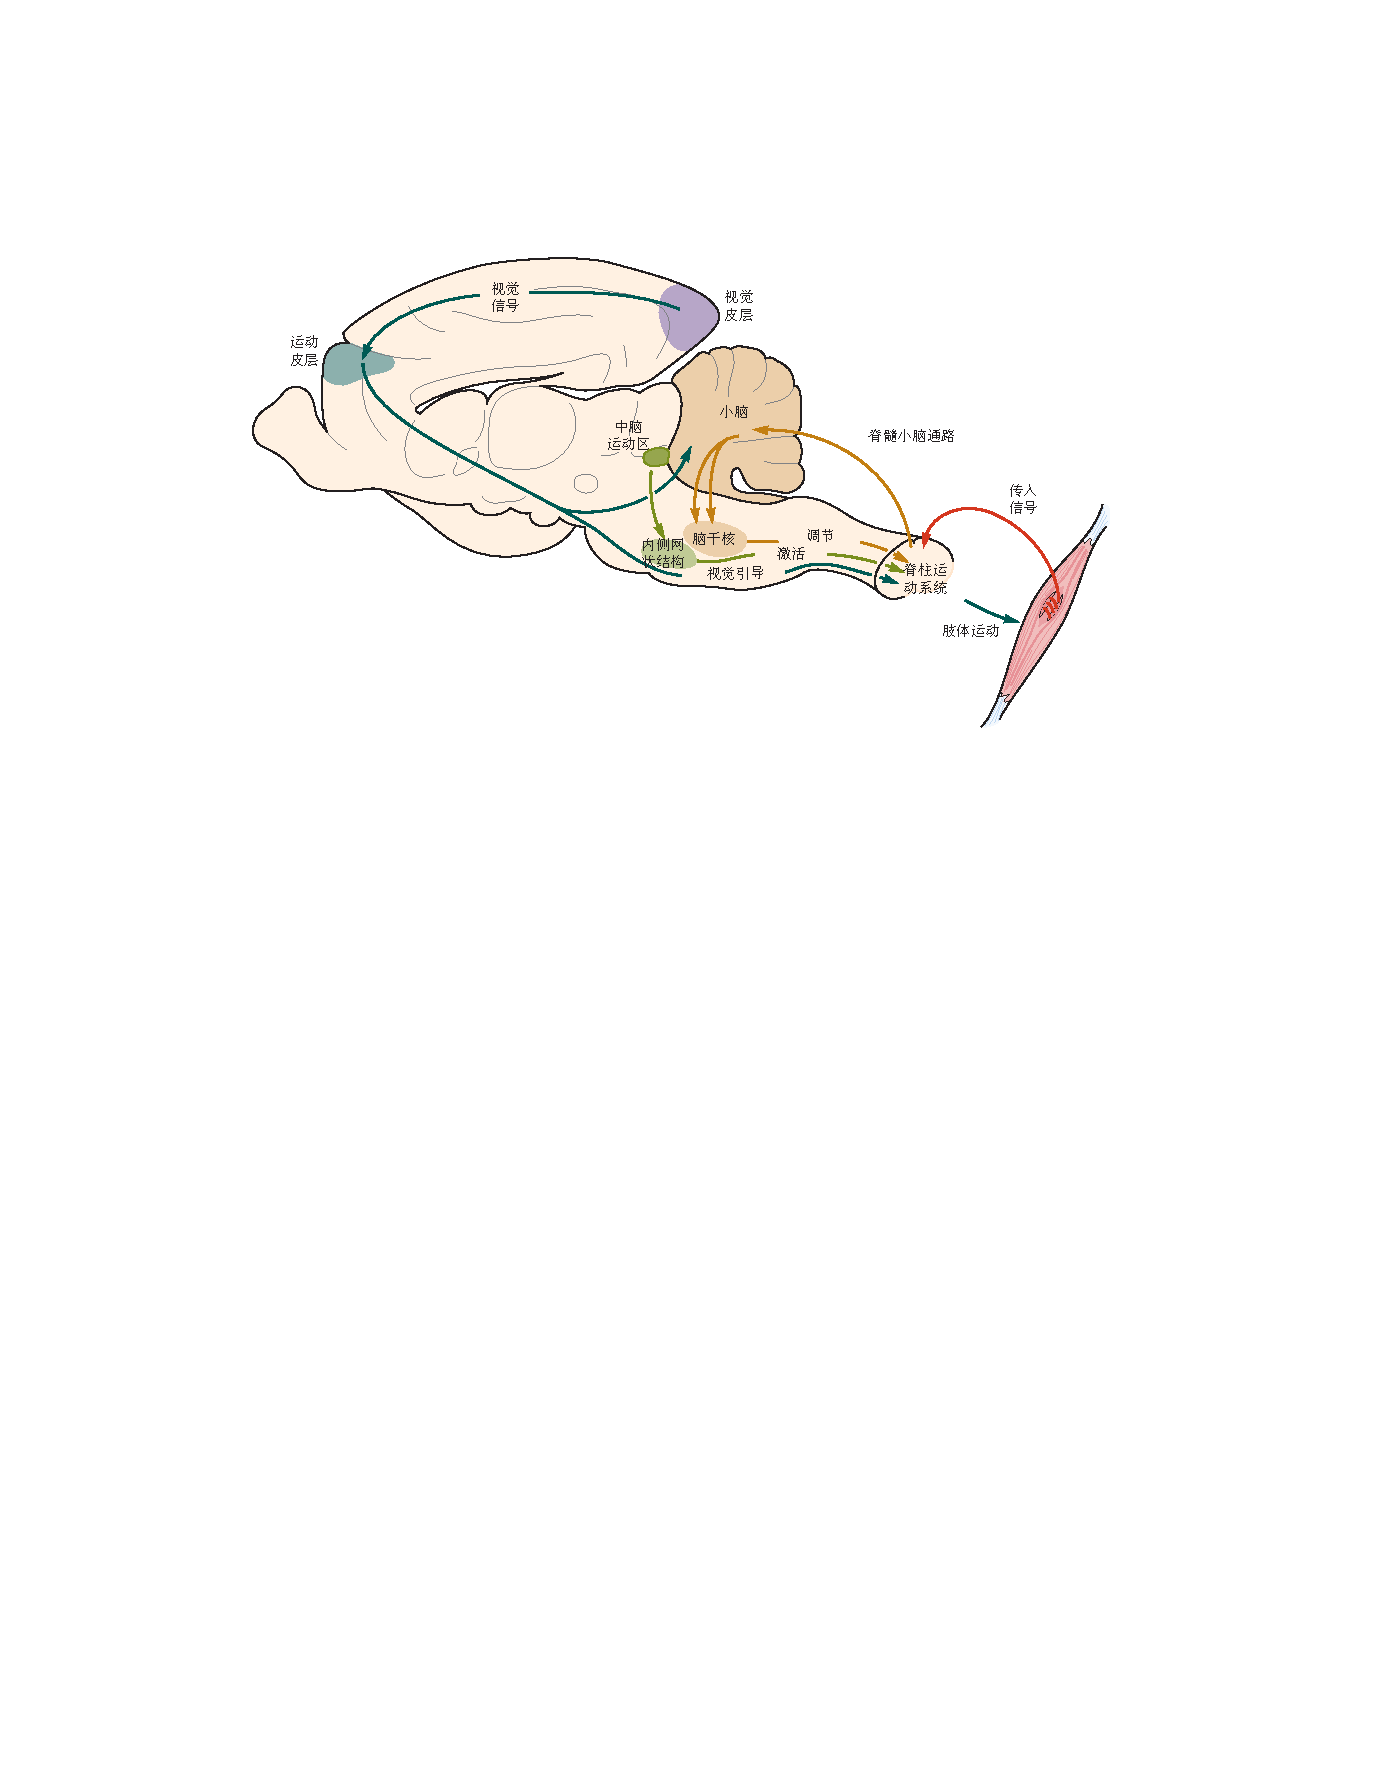
\includegraphics[width=0.85\linewidth]{chap33/fig_33_1}
	\caption{运动系统。 中枢神经系统的多个区域相互作用以启动和调节运动。 脊髓中的运动网络——中央模式发生器 (CPG)——产生精确的运动时间和模式。 本体感觉反馈调节运动 CPG 的活动。 运动的启动由中脑运动区 (MLR) 中的神经元介导,这些神经元投射到下脑干中的内侧网状结构 (MRF) 中的神经元,后者又投射到脊髓。 来自前庭核、桥脑网状结构和红核(脑干核)的下行纤维保持平衡并调节正在进行的运动活动。 来自后顶叶皮层(未图示)和运动皮层的皮质活动参与视觉引导运动的规划和执行,而基底神经节(未图示)和小脑对于运动活动的选择和协调很重要。}
	\label{fig:33_1}
\end{figure}


自 20 世纪初以来,科学家们一直对运动的神经机制很感兴趣,当时 Charles Sherrington 和 Thomas Graham Brown 的开创性工作表明,猫的孤立脊髓能够产生运动活动的基本方面,随后 这种能力是脊髓固有的。
在整个 20 世纪,在详细说明脊髓的节律和模式产生能力方面取得了重大进展,最终导致了脊髓运动的中央模式发生器的开创性概念。
自 1970 年代以来,这一单一概念比其他任何概念都更能推动对运动控制机制的研究,从而允许对运动控制中涉及的神经元机制进行详细的电生理学检查,这对于大多数其他运动行为是不可能的。


整个 20 世纪大多数关于调节运动的脊柱机制的研究都是在猫身上进行的,猫仍然是研究运动控制许多方面的重要模型。
然而,哺乳动物脊髓回路的复杂性导致寻找更简单的准备工作,以便更好地了解负责运动产生的突触连接和神经元特性。
这一研究导致了七鳃鳗和蝌蚪模型的开发(方框 33-1;图 \ref{fig:33_2} 和 \ref{fig:33_3})。 
使用这些物种进行的实验导致对负责产生游泳的神经回路的详细了解。 理解运动潜在过程的有影响力的工作也来自其他实验模型,包括小鼠、大鼠、乌龟、蝾螈和斑马鱼。


\begin{figure}[htbp]
	\centering
	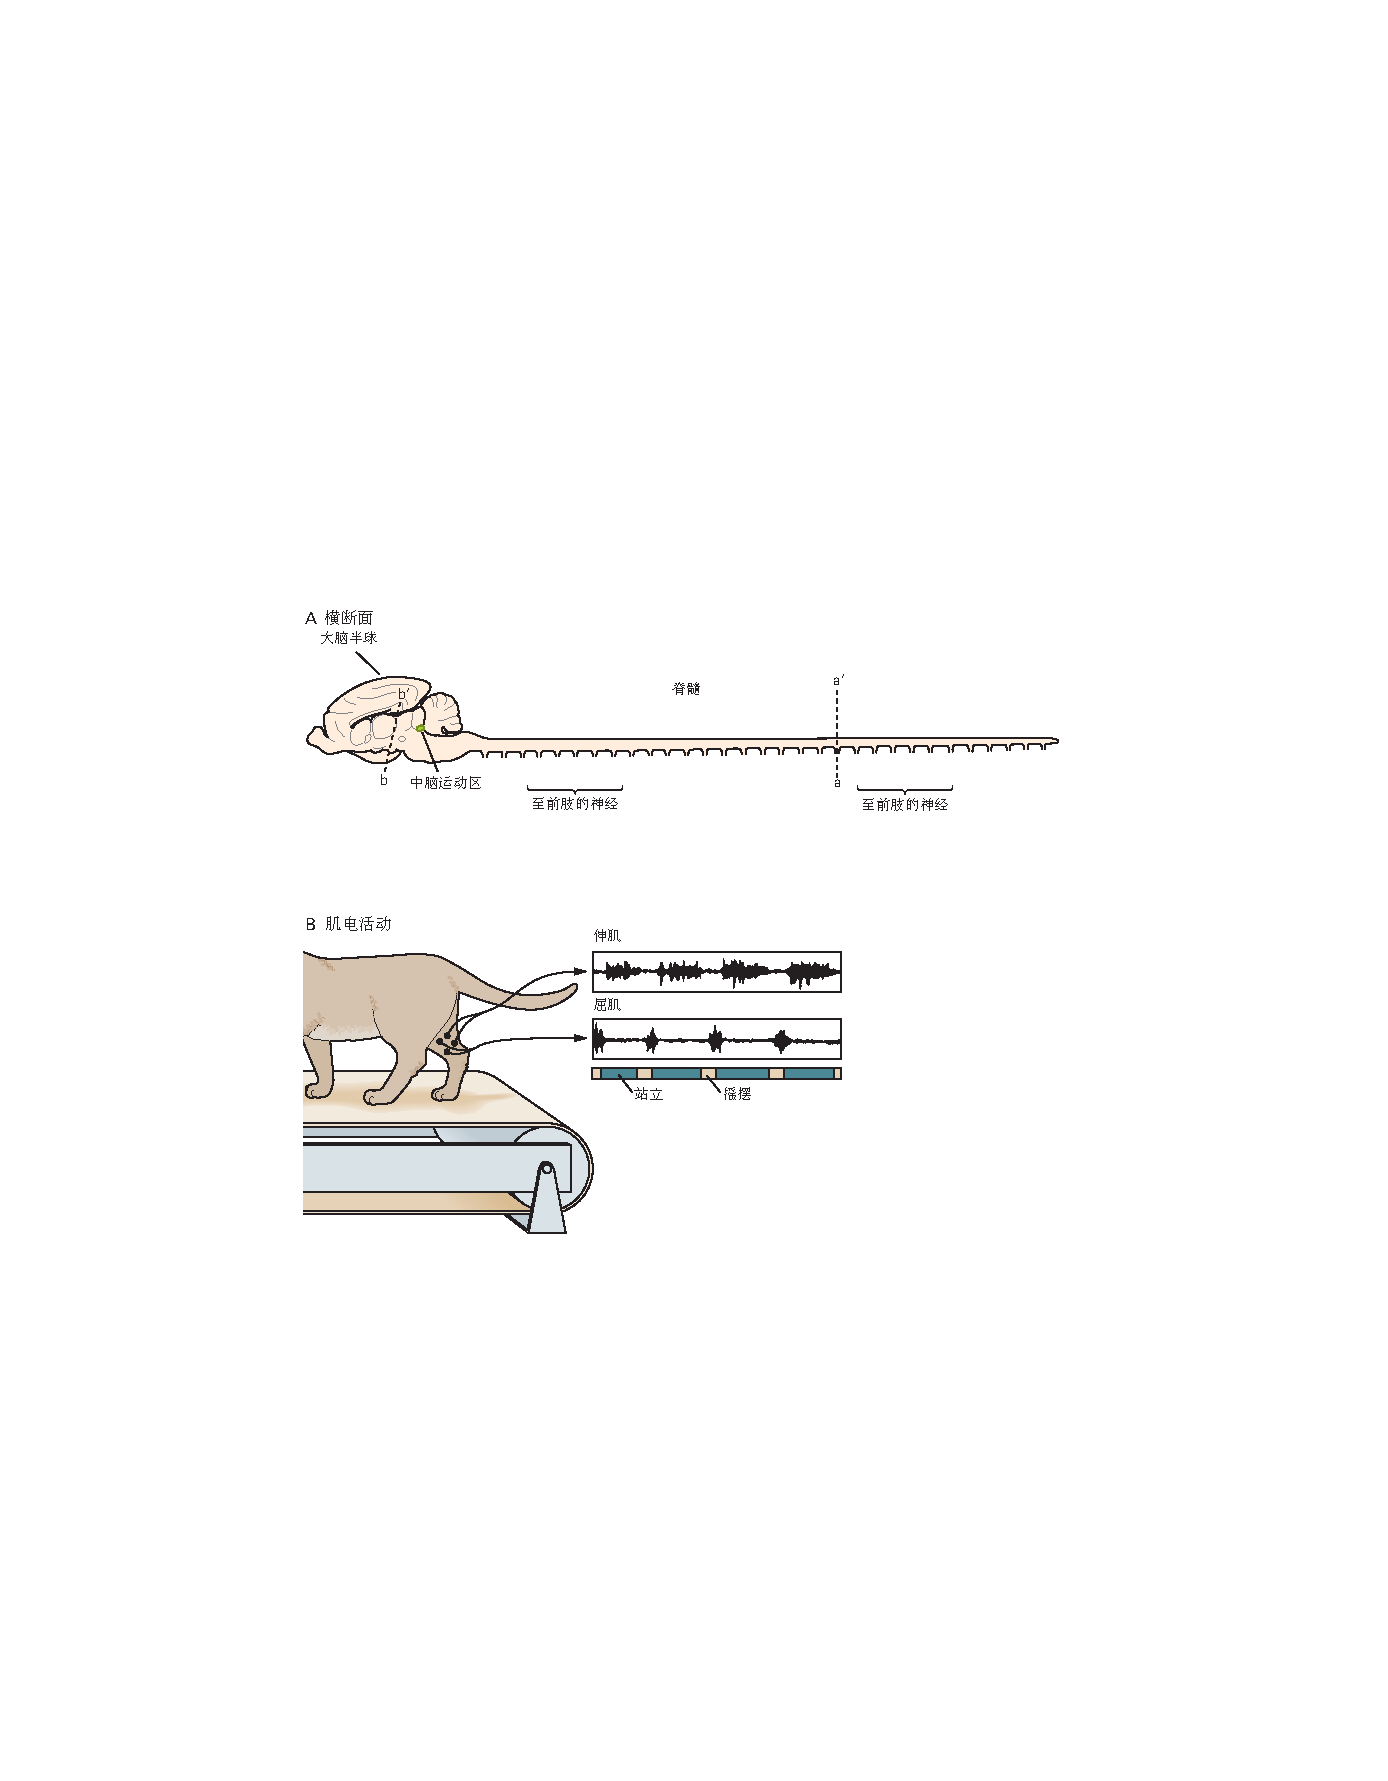
\includegraphics[width=0.7\linewidth]{chap33/fig_33_2}
	\caption{用于研究运动控制系统的选定动物模型。 A. 猫大脑半球、脑干和脊髓的示意图,显示了脊髓化 (a'-a) 和去大脑 (b'-b) 的横切水平。 去大脑将脑干和脊髓与大脑半球分离。 a'-a 处的横断面将腰椎脊髓与所有下行输入隔离开来。 B. 肌电图可用于记录完整、去大脑或脊柱动物实际运动过程中的运动活动。}
	\label{fig:33_2}
\end{figure}

\begin{figure}[htbp]
	\centering
	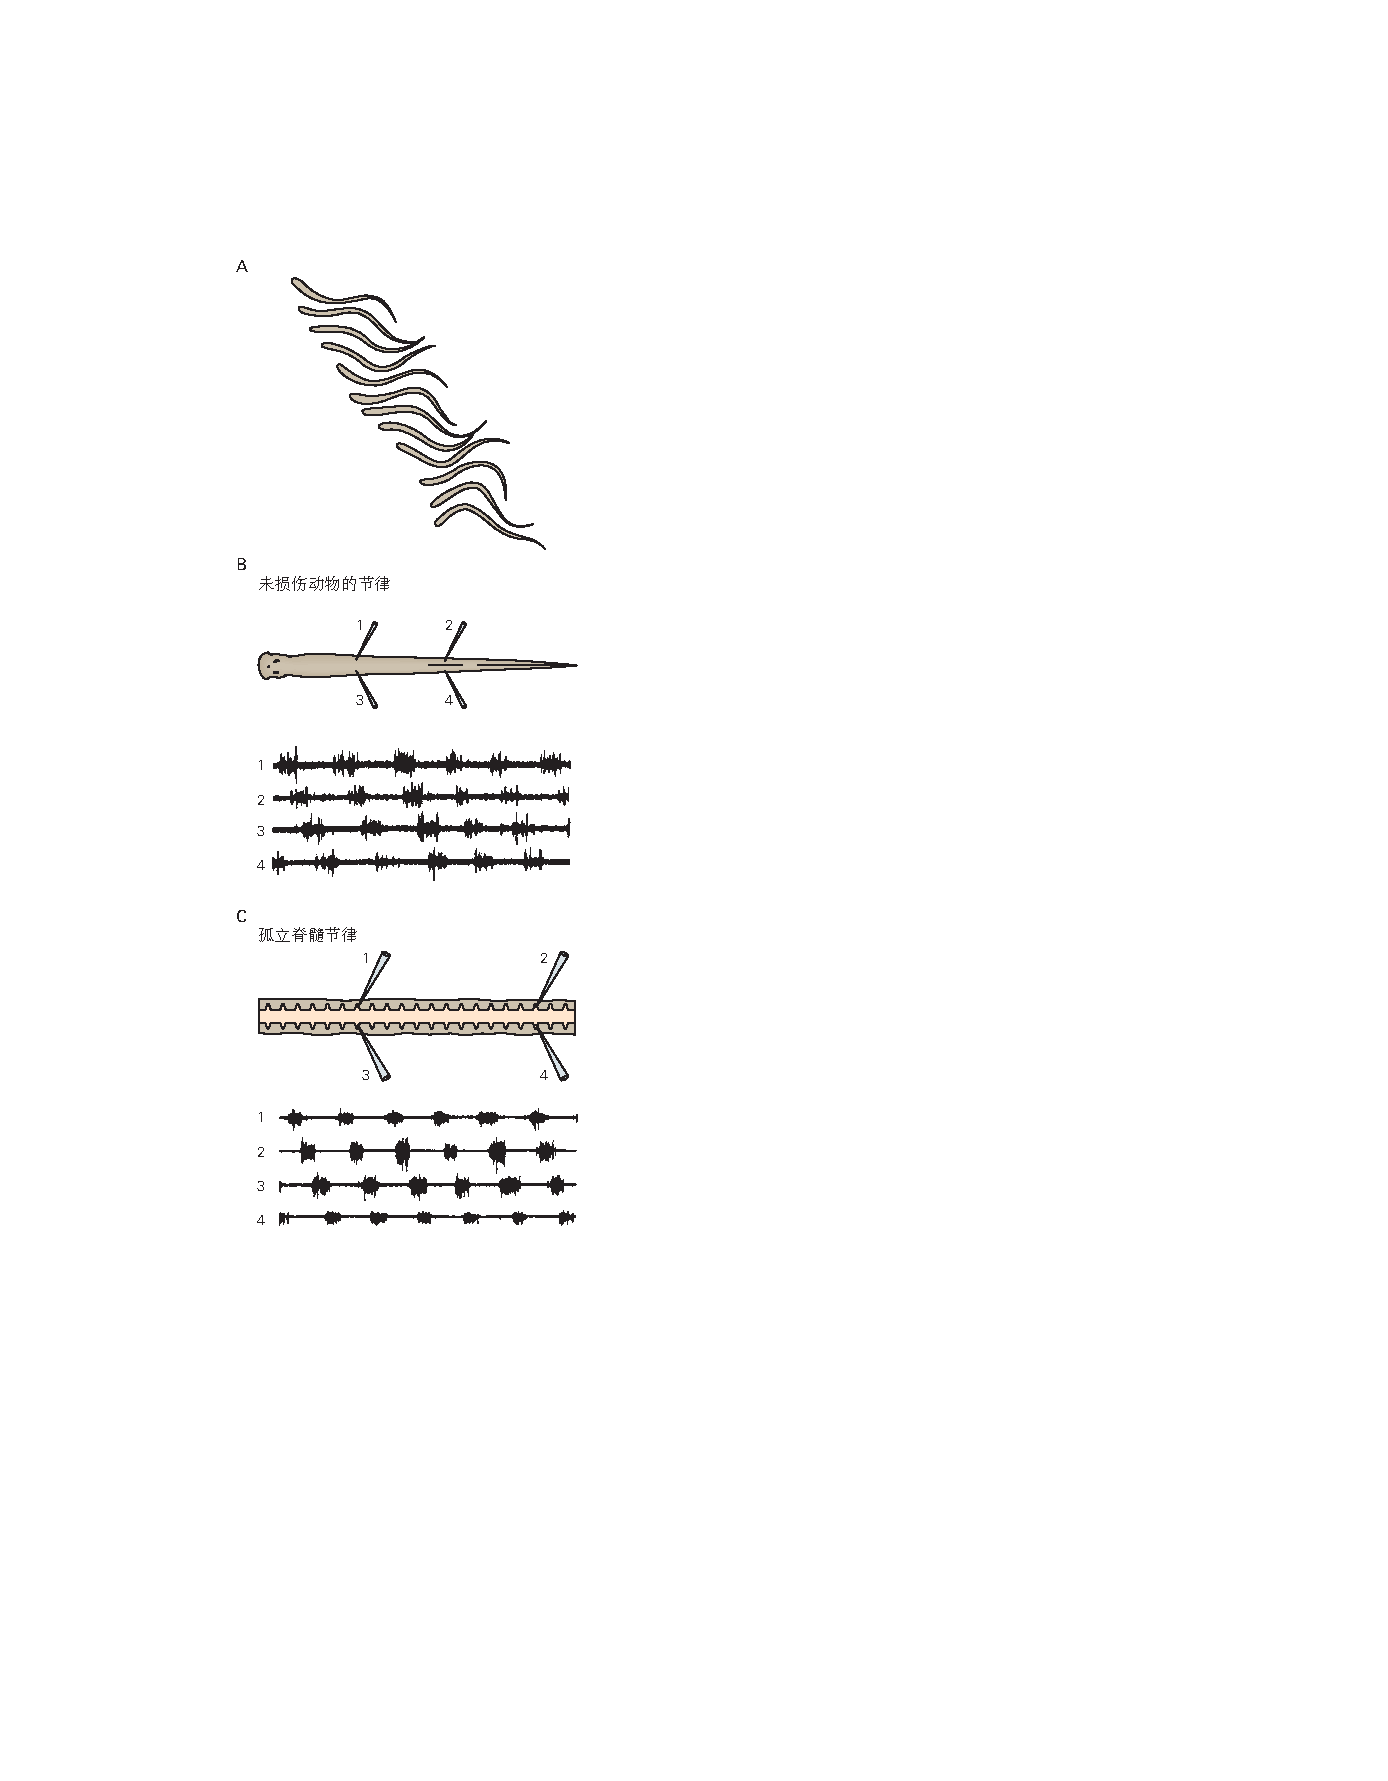
\includegraphics[width=0.4\linewidth]{chap33/fig_33_3}
	\caption{七鳃鳗游泳。 七鳃鳗通过沿着身体一侧向下移动的肌肉收缩波与另一侧的类似行进波异相 180° 进行游泳 (A)。 这种模式在动物正常游泳期间四个位置的肌电图记录中很明显 (B)。 从孤立的索 (C) 中的四个腹根记录了类似的模式。 (来自 S Grillner 的数据。)}
	\label{fig:33_3}
\end{figure}

最近,分子遗传学技术的发展提供了一种强大的工具来探测负责运动的脊髓回路,如斑马鱼和小鼠。
这些技术使研究人员能够更彻底地探索哺乳动物脊髓中负责有节奏、交替活动模式的神经元回路,这些活动模式定义了地面运动和负责游泳的活动。


活动的节奏模式只是在大多数脊椎动物中观察到的复杂运动行为的一个要素,尤其是哺乳动物,它们已经进化到可以快速优雅地移动。
这种灵活性是通过脊柱网络生成的运动模式的反馈和前馈修改提供的。


来自身体和四肢的皮肤和本体感受输入形式的反馈信息对于调节运动周期的各个方面非常重要,包括身体弯曲、步幅长度和推进过程中产生的力。
这些信息对于确保动物能够快速有效地对环境中的意外扰动做出反应同样至关重要,例如在行走过程中撞到树枝或踩到不稳定的表面时。


来自脊髓上系统的前馈信息根据动物的目标和它移动的环境修改活动。
来自脑干中定义结构的信息对于运动的启动和运动活动的一般方面的调节都很重要,包括运动速度、肌肉活动水平和具有四肢的动物的肢间耦合。
来自皮层结构的信息主要有助于在视觉用于对步态进行预期修改的情况下运动的规划和执行。
最后,基底神经节和小脑这两个没有直接脊柱连接的结构有助于运动活动的选择及其协调(图 \ref{fig:33_1})。


所有这些结构相互作用并允许不同运动模式的方式是本章的主题。



\section{运动需要产生精确协调的肌肉激活模式}

运动需要在许多肌肉中产生活动,这些肌肉需要以精确的节奏和模式进行协调。
节奏定义了循环活动的频率,而模式定义了一个周期内肌肉群的时空激活。
在游泳动物中,如七鳃鳗或蝌蚪,运动表现为活动的行波(图 \ref{fig:33_3}A),在向前进展过程中从头肢体节传播到尾肢体节。
这种模式可以记录为完整动物运动期间的肌电图 (EMG)(图 \ref{fig:33_3}B)和分离脊髓中的神经电图(图 \ref{fig:33_3}C)。
更多尾根的活动发生在更多尾根中,并且身体两侧的活动是相互的。


在有肢动物中,肌肉活动的模式更为复杂,用于支撑身体并向前移动。
有肢脊椎动物运动的一般测量单位是步周期,它被定义为任何两个连续事件之间的时间(例如,给定肢体的脚或爪子接触)。
步伐周期分为摆动阶段,当脚离开地面并向前移动时,以及站立阶段,当脚与地面接触并推动身体向前移动时。
根据关节角度变化的测量,这些阶段中的每一个都可以进一步分为屈曲期 (F),随后是摆动期的初始伸展期 (E1) 和站立期的两个额外伸展期 (E2 和 E3) (图 33–4A;见下文)。


必须以精确的时空模式激活和协调单个肢体中的肌肉(图 \ref{fig:33_4}B),以便协调不同肌肉激活的相对时间、活动持续时间和活动强度以满足需求 环境(肢内协调)。


\begin{figure}[htbp]
	\centering
	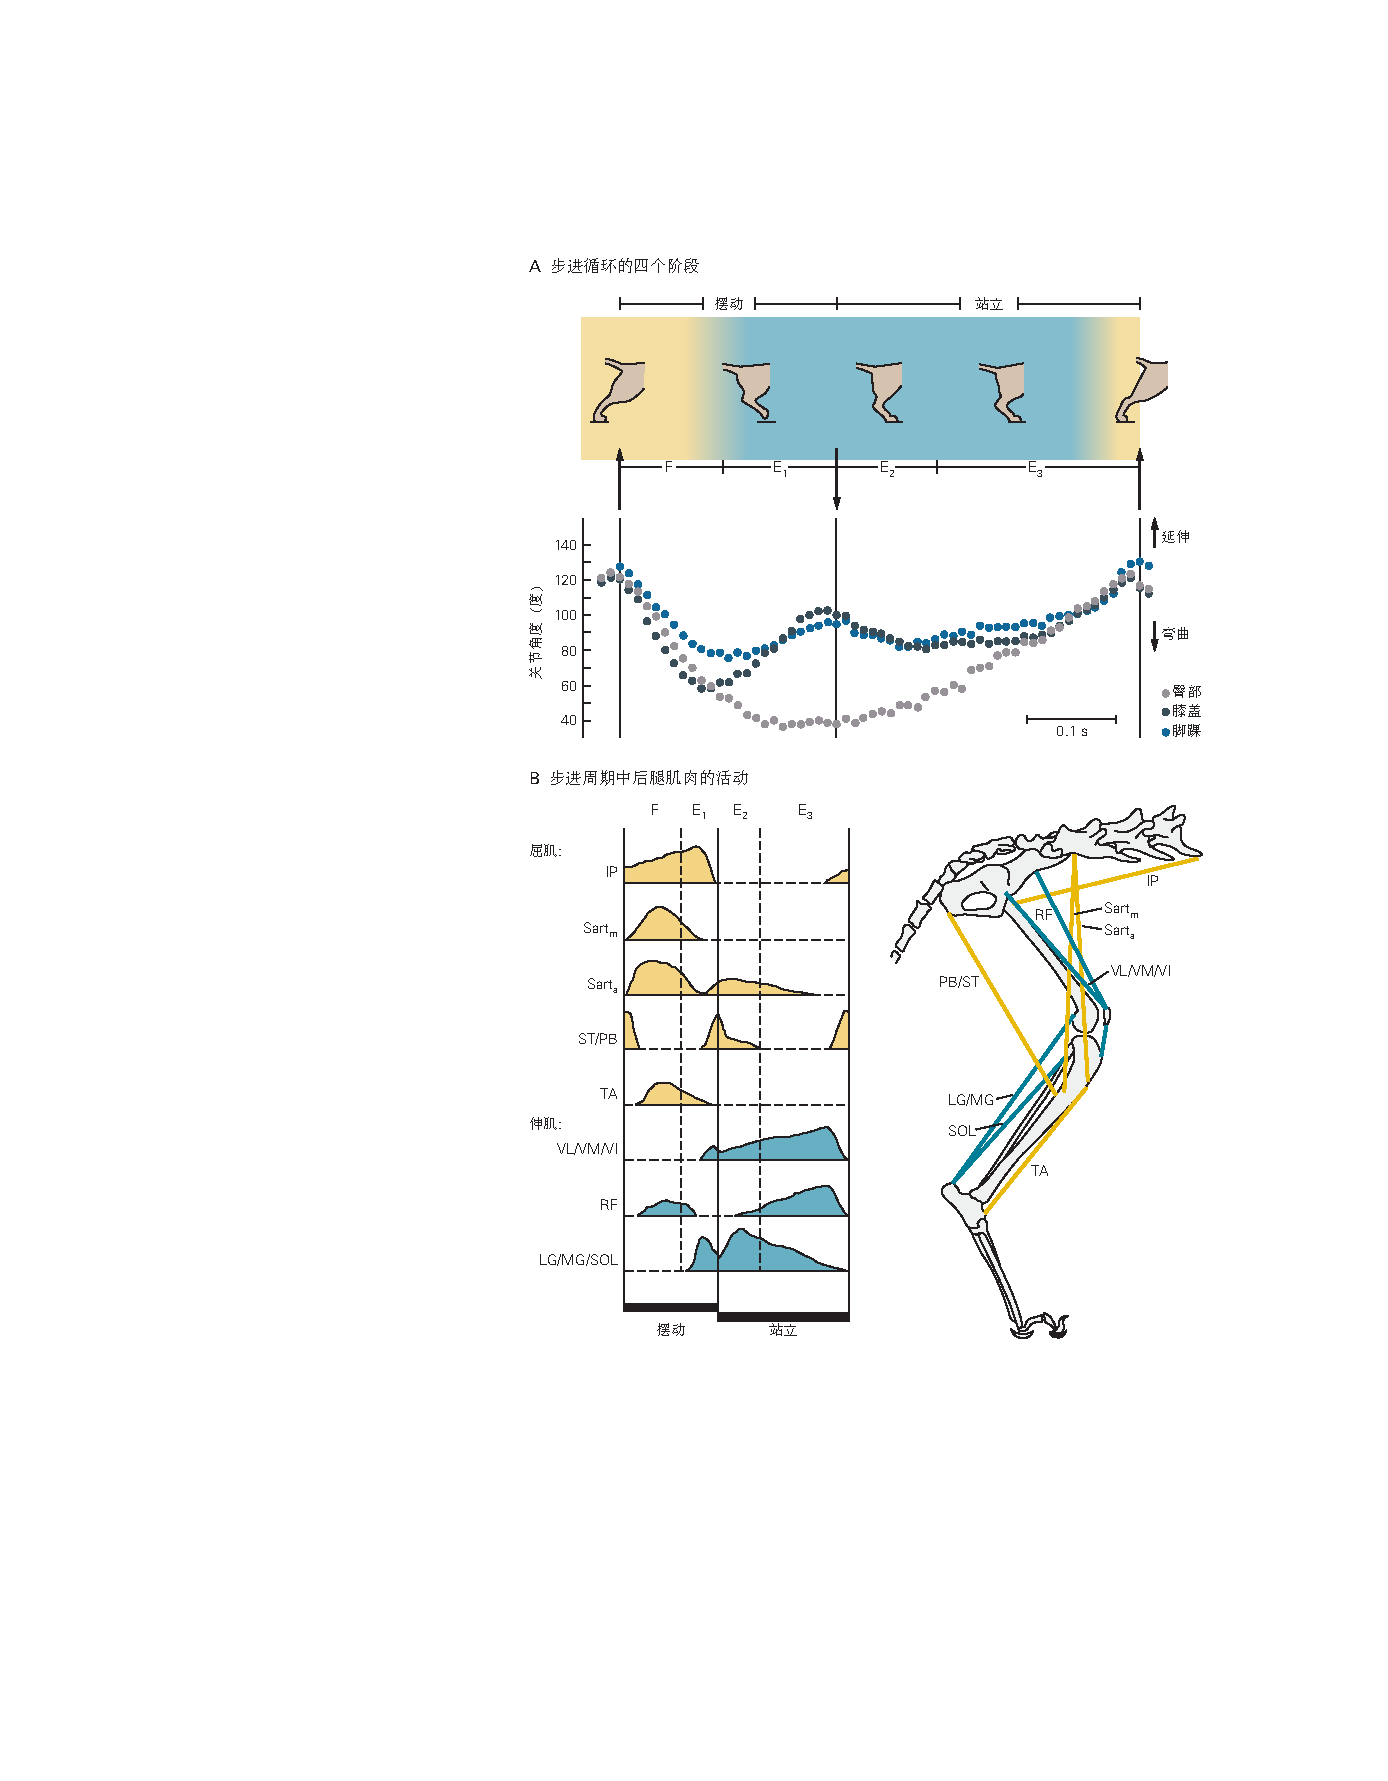
\includegraphics[width=0.65\linewidth]{chap33/fig_33_4}
	\caption{迈步是由腿部肌肉收缩的复杂模式产生的。 A.步循环分为四个阶段。 屈曲 (F) 和第一次伸展 (E1) 阶段发生在摆动阶段,此时脚离开地面,而第二次伸展 (E2) 和第三次伸展 (E3) 发生在站立阶段,当脚接触地面时 . E2 的特点是膝盖和脚踝弯曲,因为腿开始承受动物的重量。 收缩的膝关节和踝关节伸肌在此阶段伸长。 (经许可改编自 Engberg 和 Lundberg 1969。)B. 猫在行走过程中一些后腿屈肌(黄色)和伸肌(蓝色)的电活动曲线。 虽然屈肌和伸肌通常分别在摆动和站立阶段活跃,但总体活动模式在时间和幅度上都很复杂。 (肌肉:IP,髂腰肌;LG 和 MG,外侧和内侧腓肠肌;PB,后二头肌;RF,股直肌;Sartm 和 Sarta,内侧和前缝匠肌;SOL,比目鱼肌;ST,半腱肌;TA,胫骨前肌;VL, VM 和 VI、股外侧肌、股内侧肌和股中间肌。)}
	\label{fig:33_4}
\end{figure}


在后肢中,摆动是由激活半腱肌等肌肉产生的膝关节屈曲引发的,紧接着是髋屈肌和踝屈肌的激活(F 期)。
髋屈肌在整个摆动过程中持续收缩,但膝屈肌和踝屈肌的活动在腿部伸展以准备与支撑面接触时停止(E1 阶段)。
大多数伸肌的活动在这个阶段开始,在脚接触地面之前。
这个准备阶段表明伸肌活动是集中编程的,而不仅仅是脚与地面接触所产生的传入反馈的结果。


姿势从脚或爪子与地面接触开始。 在站立早期(E2 阶段),膝关节和踝关节因承受身体重量而弯曲,导致伸肌在强烈收缩(离心收缩)的同时伸长。
当承受重量时,这些肌肉会像弹簧一样屈服,使身体能够在脚上平稳移动,这对于建立有效的步态至关重要。
在站立后期(E3 阶段),臀部、膝盖和脚踝都伸展,因为伸肌提供推动力使身体向前移动。


还需要肢间协调,即不同肢体之间的精确耦合。
例如,四足动物的四条腿之间的耦合可能会有很大差异,这取决于运动速度和采用的步态(步行、步伐、小跑、疾驰或跳跃)。
对于同侧肢体(同侧肢体)和对角肢体的肌肉之间的耦合模式尤其如此。
肢体之间的关系可以用相位差来表征,其中 0 个反射肢体同相移动,0.5 个肢体完全异相移动(即,在相反的方向)。
行走过程中,同侧肢体之间的活动以0.25的相位值变化,三条腿始终与地面接触。 小跑时,对角线肢体(如左后肢和右前肢)同相,同侧肢体的相位差为0.5。 与同步运动相比,同一腰带的四肢(即前肢或后肢)之间的相位关系在交替肢体激活产生的步态期间更稳定,例如步行或小跑(通常异相 0.5 个周期) 疾驰或奔跑(通常是同步的)。


活动的肢内和肢间协调的适当产生以及根据环境适应这些活动模式是中枢神经系统在运动过程中的主要功能之一。



\section{踏步的运动模式是在脊髓水平组织的}

虽然整个神经系统对于动物产生丰富的行为库是必要的,但脊髓足以产生运动的节奏以及肢内和肢间协调所需的许多特定肌肉活动模式。


20 世纪初,格雷厄姆·布朗 (Graham Brown) 表明,在脊髓没有感觉输入的情况下,孤立的脊髓具有在踝关节周围产生基本交替运动模式的内在能力(图 \ref{fig:33_5})。
他提出控制脊髓屈肌和伸肌活动的运动网络被组织为半中心,这样当电路的一半处于活动状态时,它会抑制另一半。 该中心将通过某种突触或神经元疲劳从抑制中释放出来。


\begin{figure}[htbp]
	\centering
	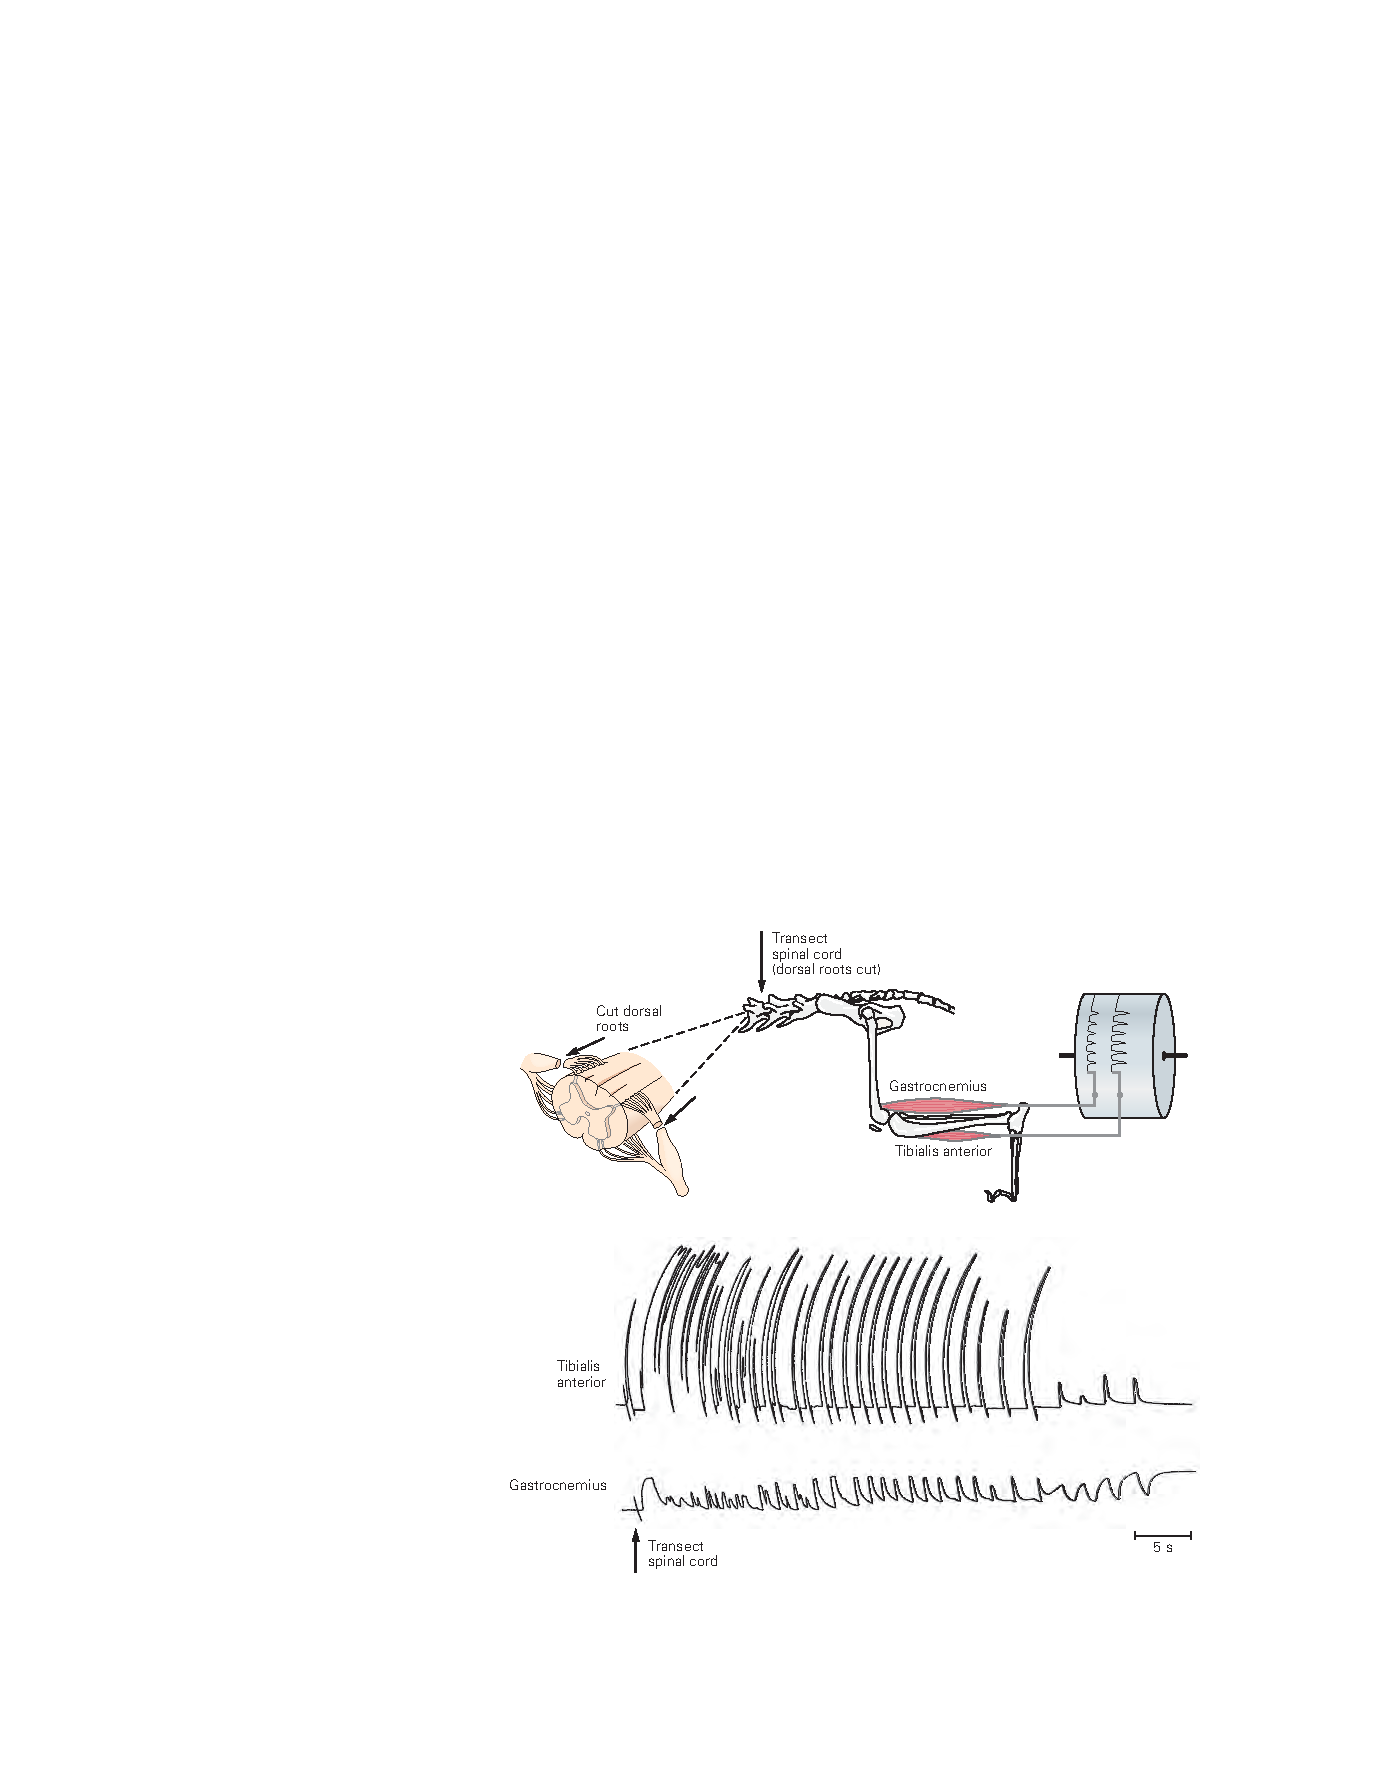
\includegraphics[width=0.7\linewidth]{chap33/fig_33_5}
	\caption{有节奏的步进是由脊柱网络产生的。 1911 年,托马斯·格雷厄姆·布朗 (Thomas Graham Brown) 首次证明了内在脊柱网络的存在,他开发了一种实验制剂,在该制剂中,背根被切断,因此来自肢体的感觉信息无法到达脊髓。 下图显示了格雷厄姆·布朗 (Graham Brown) 研究中的原始记录。 踝关节屈肌(胫骨前肌)和踝关节伸肌(腓肠肌)的节律性交替收缩由孤立的脊髓产生,并在横断后持续一段时间。}
	\label{fig:33_5}
\end{figure}

直到 20 世纪 60 年代中期和 ea 在半中心模型中,脊髓只产生运动节律,而模式是由运动引起的传入反馈塑造的,这一开创性的观察大多被忽视。 
然而,这种观点被实验改变了,实验表明在背根部分后在跑步机上行走的去大脑和脊椎猫可以观察到组织良好的运动模式,从而消除传入反馈(图 \ref{fig:33_6}A,B)。 
后来在慢性脊髓猫身上进行的实验通过阻止运动来消除节律性传入反馈(图 \ref{fig:33_6}C),表明脊髓回路不仅能够在本质上产生运动节律,而且还可以产生一些 rly 1970s,当有一个时期开始时 深入研究脊髓产生节律活动模式的机制。
初步研究表明,用 L-DOPA(单胺递质多巴胺和去甲肾上腺素的前体)和烟酰胺(一种延长 L-DOPA 作用的药物)治疗的脊髓猫的感觉纤维刺激可以在屈肌中产生短序列的节律性活动 和伸肌运动神经元。
进一步发现,脊髓中的中间神经元组以相互屈肌和伸肌模式被激活。
这种组织特征与格雷厄姆布朗的理论一致,即相互抑制的半中心在屈肌和伸肌运动神经元中产生交替爆发活动。
在完整猫中观察到的活动模式的时空细节(图\ref{fig:33_6}C)。


\begin{figure}[htbp]
	\centering
	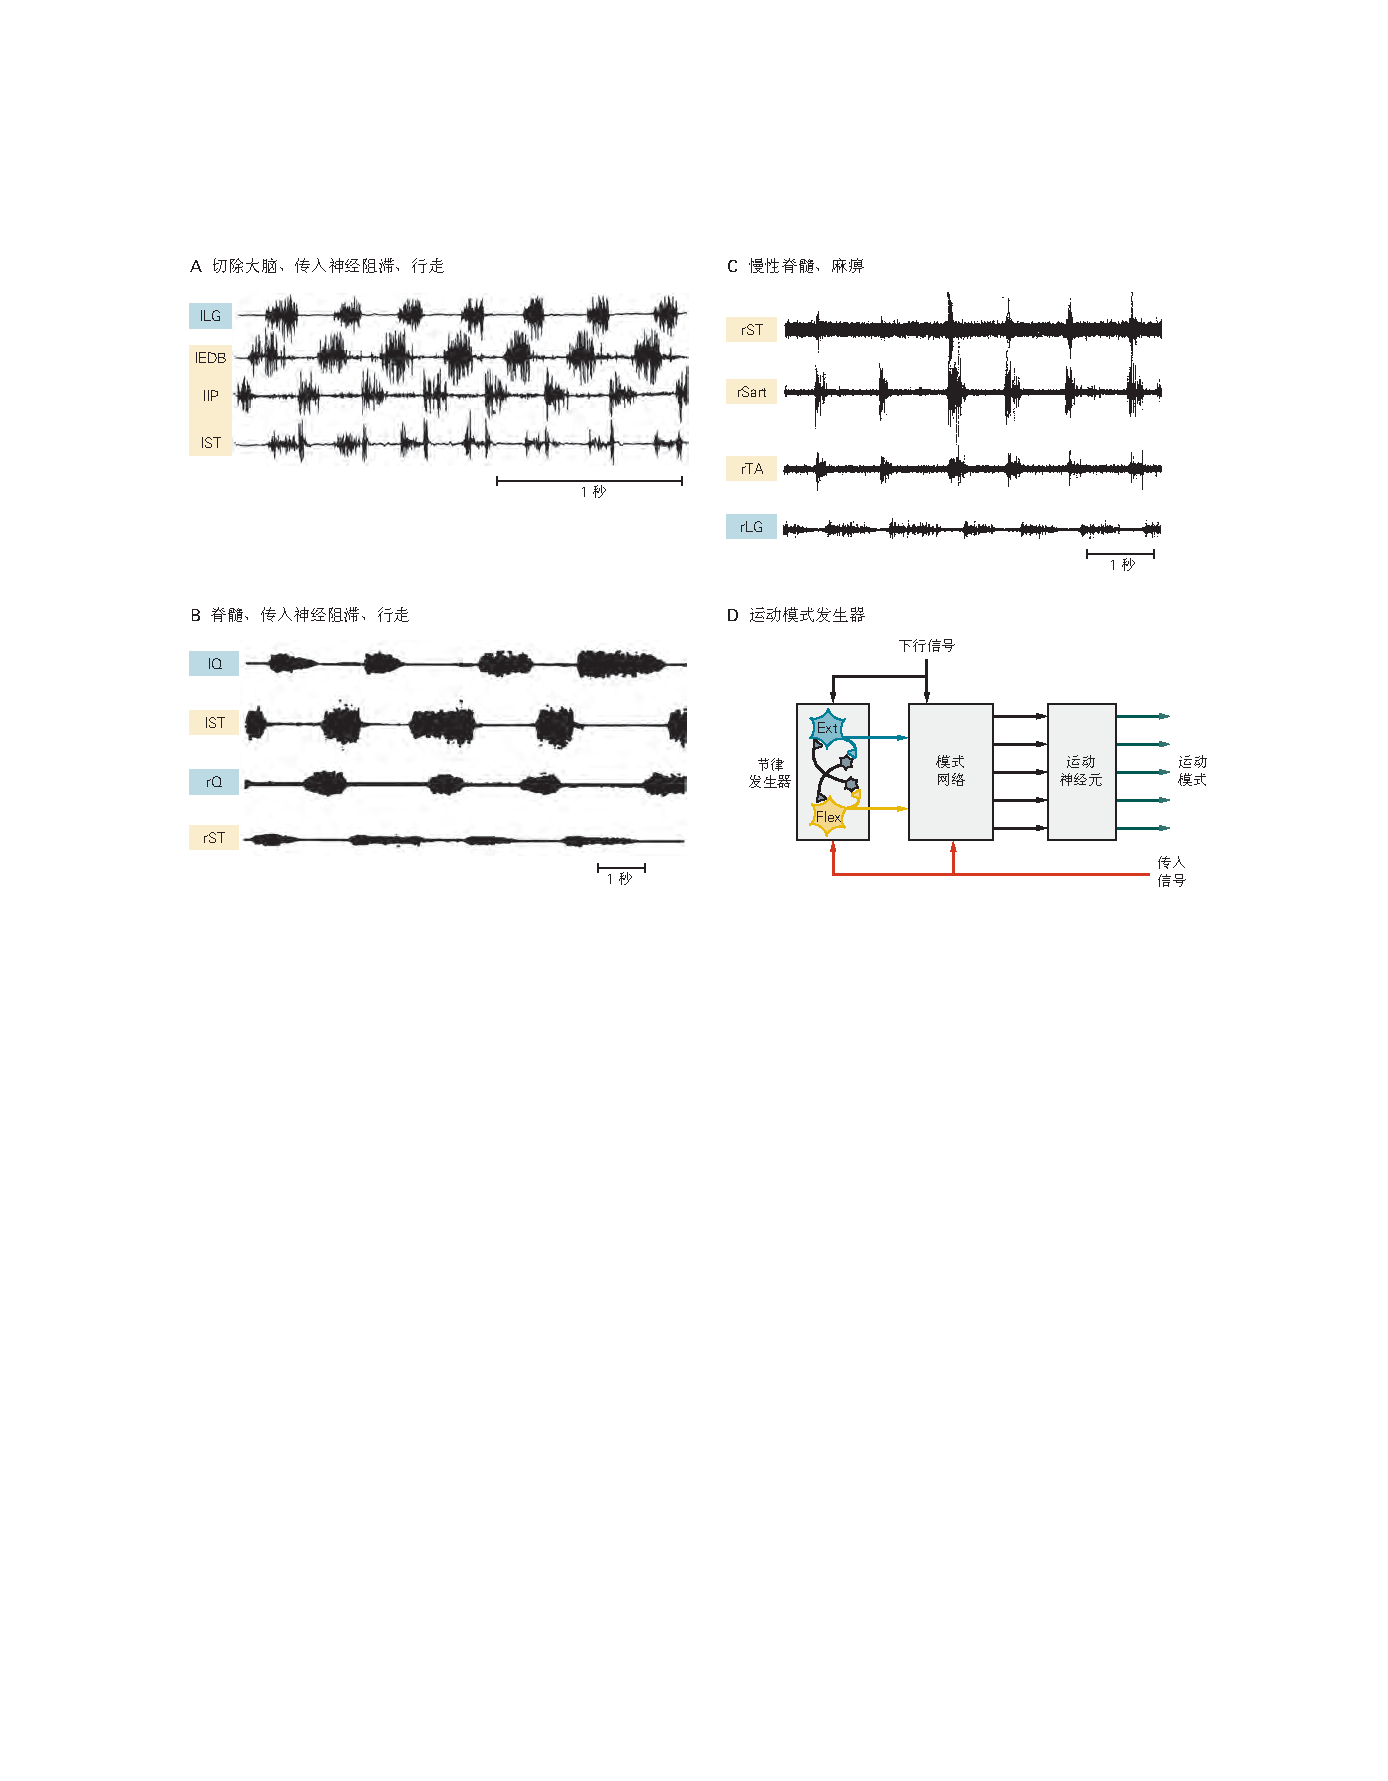
\includegraphics[width=0.95\linewidth]{chap33/fig_33_6}
	\caption{脊髓回路产生节奏和模式。 A. 即使在通过切断背根去除了脊髓的所有感觉输入之后,在跑步机上行走的去大脑猫表现出复杂的运动模式,而不仅仅是屈肌和伸肌活动的简单交替。 (缩写:l,左;EDB,趾短伸肌;LG,腓肠肌外侧;IP,髂腰肌;ST,半腱肌。)(经许可改编自 Grillner 和 Zangger 1984。)B. 左旋多巴和烟酰胺的静脉注射 在背根被切断的急性脊柱猫中产生组织良好的运动模式。 (缩写:l,左;Q,股四头肌;r,右。)(经 Grillner 和 Zangger 1979 许可改编。版权所有 © 1979 Springer Nature。)C. 慢性脊髓瘫痪猫的虚构运动,展示典型的活动模式 在完整猫的半腱肌、胫骨前肌 (TA)、腓肠肌外侧 (LG) 和缝匠肌 (Sart) 中。 (l,左;r,右。)(改编自 Pearson 和 Rossignol 1991。)D. 基于去大脑猫研究的脊髓运动中枢模式发生器 (CPG) 的概念模型。 CPG 模型由单独的节奏和模式生成层组成。 这些层中的每一层都可以通过下行输入和外围传入信息进行修改。 (改编自 Rybak 等人,2006 年。)}
	\label{fig:33_6}
\end{figure}

这些观察导致了中央模式发生器 (CPG) 的重要概念,它可以独立于感官输入生成节奏和模式。 随后的实验导致了这样的想法,即 CPG 的独立组件负责产生肢体运动的潜在节奏和肢体肌肉动作的时空模式(图 \ref{fig:33_6}D)。
这个概念是基于这样的观察,即节奏和模式的变化可以独立受到影响。
其他研究提出了 CPG 是模块化的概念,允许独立控制不同关节周围的活动。


对各种物种的实验表明,每个肢体可能都有单独的 CPG。
例如,使用分离带的实验表明,动物可以独立地修改每对肢体的步进周期持续时间,其中前后肢或左右肢在单独的跑步机带上行走。
该组织将允许相对简单的下降命令来修改每个 CPG 之间的耦合,从而改变步态的模式。


现在已经在许多有节奏的运动系统中识别和分析了 CPG,包括那些控制无脊椎动物和脊椎动物的地面运动、游泳、飞行、呼吸和吞咽的运动系统。
在除高等灵长类动物和人类以外的所有脊椎动物中,在脊柱横断后立即可以观察到明显的运动模式,此时横断处下方的脊髓被神经活性药物激活,这些药物替代了通常激活脊髓运动网络的下行驱动(方框) 33-1)。


\subsection{负责运动的脊髓回路可以根据经验进行修改}

其他方面完好的成年哺乳动物的脊髓损伤会导致瘫痪。 在没有任何进一步干预的情况下,这些动物将只能恢复最小的运动能力。
然而,当每天训练胸脊髓完全损伤的四足动物时,它们会重新获得使用后肢在跑步机上行走的非凡能力。


应用去甲肾上腺素能激动剂也可以获得类似的运动改善。
事实上,这些动物的后肢关节角度和 EMG 活动的记录表明,从所有下行系统中分离出来的脊髓可以在完整动物中观察到的后肢中产生大部分协调特征。
这种训练效果被认为是由于内部脊髓回路的活动依赖性重组和来自外周传入的突触输入的修改而发生的,这是训练方案特有的。
事实上,可以专门训练猫来支撑它们的体重或走路,而无需在这两种行为之间转移运动技能。




\subsection{脊髓运动网络被组织成节奏和模式生成电路}

脊髓如何产生运动背后的复杂活动的问题一直是遵循三个互补路径的深入研究之一。
最早针对这个问题的实验是在猫身上进行的,并提供了关于不同神经元间群体功能特征的重要信息。
然而,哺乳动物脊髓的复杂性促使研究人员确定了脊髓中神经元较少的模型,例如乌龟和两种水生生物,即蝌蚪和七鳃鳗(方框 33-1)。
后两种模型为了解游泳中涉及的脊髓回路的组织提供了一个极好的窗口,并为研究四肢动物的节律和模式生成奠定了基础。
最后,小鼠和斑马鱼重要分子遗传模型的发展提供了更传统方法无法获得的更多见解。


游泳中央模式发生器

七鳃鳗——一种无颌鱼——像鳗鱼一样游动,从前到后左右弯曲(图 \ref{fig:33_3}A)。
脊髓由大约 100 个脊髓节段组成,每个节段都包含神经元,可以产生节律并在身体两侧产生交替。
节律是由相互连接的谷氨酸能兴奋性神经元产生的,这些神经元具有支持节律产生的活性膜特性。
这些谷氨酸能神经元是游泳网络的核心,它们会刺激脊髓同一侧的连合抑制神经元、局部抑制神经元和运动神经元(图 \ref{fig:33_7}A)。


\begin{figure}[htbp]
	\centering
	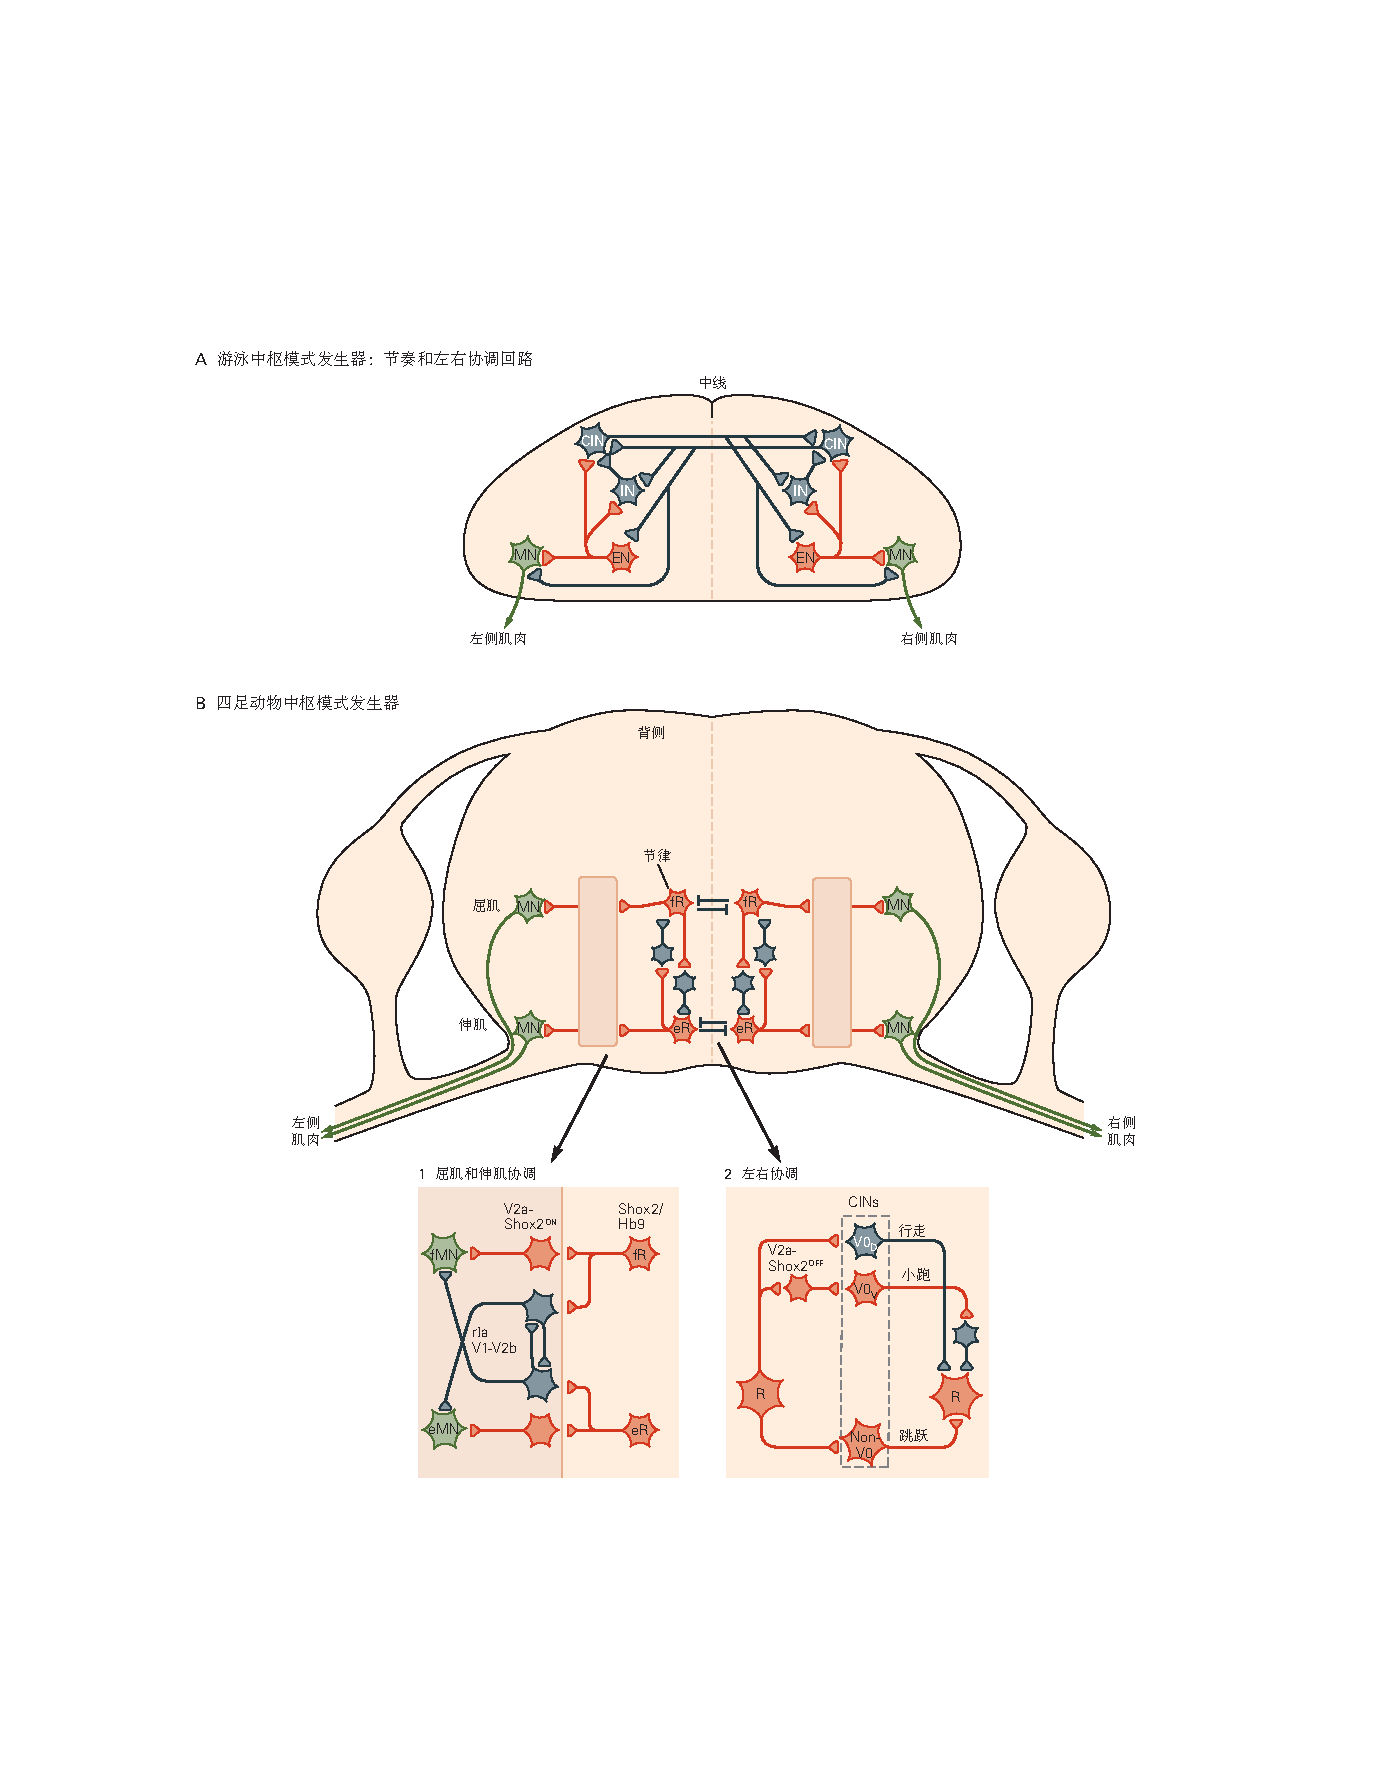
\includegraphics[width=0.8\linewidth]{chap33/fig_33_7}
	\caption{脊髓运动网络被组织成具有不同细胞身份的节律和模式生成回路。 A. 七鳃鳗游泳中央模式发生器 (CPG) 的电路图。 节律产生回路包括驱动运动神经元 (MN) 的兴奋性中间神经元 (EN)、轴突投射到脊髓另一半的抑制性连合中间神经元 (CIN),以及轴突投射在脊髓同一侧的局部抑制性中间神经元 (IN) 电源线。 图中的单个神经元代表动物体内的多个神经元。 灰色神经元,抑制性; 红色神经元,兴奋。 垂直虚线表示中线。 (数据来自 Grillner 2006。) B. 四肢运动的一般电路图。 由脊髓两侧的兴奋性神经元组成的节律生成回路(fR 和 eR)通过模式生成层(空框)驱动同一侧的屈肌和伸肌。 产生节律的屈肌 (fR) 和伸肌 (eR) 神经元通过抑制性神经元相互连接,并通过调节左右协调的连合中间神经元(未显示)跨中线连接。 该图显示了一个脊柱节段。 (缩写:MN,运动神经元。)(数据来自 Kiehn 2016。)B1。 屈肌和伸肌交替在运动网络中的多个级别进行控制。 远离屈肌 (f) 和伸肌 (e) 运动神经元 (MN) 的一个突触是 Ia 抑制性中间神经元,它们相互支配拮抗运动神经元和彼此(第 32 章)。 rIa 神经元属于腹侧脊髓中分子定义的两大类抑制性神经元 V1 和 V2b。 具有不同分子标记(包括 V2a-Shox2ON)的兴奋性神经元提供运动神经元的运动前节律性兴奋。 产生节律的 Shox2ON 或 Hb9 神经元(fR 和 eR)驱动抑制性和兴奋性运动前神经元。 (数据来自 Kiehn 2016。) B2。 节律产生电路驱动左右协调电路,该电路由涉及交替的双重抑制通路和涉及同步的单一兴奋通路组成。 双抑制通路由直接抑制另一侧节律生成的抑制性 V0D 连合神经元和间接抑制另一侧运动网络的兴奋性 V0V 连合神经元组成。 抑制性 V0D 连合神经元通路控制交替步态行走。 一群 V2a 兴奋性神经元是左右交替电路的一部分,并连接到 V0V 连合神经元。 该通路控制交替步态小跑。 节奏生成电路还驱动可能参与绑定的左右同步电路,由非 V0 神经元组成。 仅显示从左侧到右侧的投影。 (数据来自 Kiehn 2016。)}
	\label{fig:33_7}
\end{figure}

轴突穿过中线的连合中间神经元抑制参与产生交替节律的对侧中间神经元以及对侧运动神经元(图 \ref{fig:33_7}A)。
蜂窝机制有助于网络中的相位切换(方框 33-2)。
例如,由谷氨酸能神经元爆发触发的 Ca2+ 进入会激活其钙激活 K+ 通道。
这些通道的打开使细胞超极化并使爆发终止。
一侧的爆发终止通过连合中间神经元激活另一侧,从而使对侧节律生成中间神经元和运动神经元变得活跃。
为了实现身体协调,节段网络通过兴奋性和抑制性神经元的长距离下行投射连接起来。
这种由相互连接的兴奋性神经元、抑制性连合神经元和用于节间协调的头尾连接梯度组成的基本组织也存在于蝌蚪中,并且可能与其他游泳物种相同。


分子和遗传方法扩展了我们对鱼类 CPG 功能组织的理解,并确定了两组谷氨酸能中间神经元——一组连合神经元和一组同侧投射神经元——它们参与节律生成但运动速度不同。
在成年斑马鱼中,节律产生回路由三种功能类别的兴奋性神经元组成,它们驱动慢速、中速和快速运动神经元池,随着游泳速度的增加,这些神经元被选择性地招募。


四足中央模式发生器

与游泳 CPG 相比,控制四足运动的 CPG 增加了组织复杂性,因为它必须产生节奏和模式,涉及四肢内不同关节周围肌肉的连续屈伸肌交替(图 \ref{fig:33_4}B),以及 前肢和后肢之间的左右协调和协调。
控制前肢的回路位于颈椎膨大区,而控制后肢的回路位于下胸椎和腰椎脊髓。


与产生有节奏的游泳活动的 CPG 一样,谷氨酸能兴奋性中间神经元参与四足节律的产生。
使用先进的小鼠遗传学以及建立在基因调节转录因子表达基础上的分子代码,这些转录因子将脊髓神经元区分为具有特定投射和递质表型的类别(方框 33-3),现在已经表明节律的核心- 啮齿动物中的生成电路包括两个不重叠的分子不同的谷氨酸能神经元组(Shox2ON 和 Hb9;图 \ref{fig:33_7}B1)。


屈肌 (f) 和伸肌 (e) 节律生成 (R) 回路通过相互抑制(图 \ref{fig:33_7}B)连接,驱动运动网络中的其他神经元进入节律性状态,并为运动神经元提供节律性兴奋(图 \ref{fig:33_7}B)。
正如在游泳 CPG 中观察到的那样,离子通道也可能有助于四足 CPG 中的节律生成和相位切换。


屈伸肌协调回路

屈肌和伸肌的活动必须围绕关节(例如,后肢的髋膝踝趾)进行协调,以精确地控制肢体运动。
因此,不同关节周围的屈肌-伸肌交替不是同时发生的,而是具有顺序模式,这表明需要多个屈肌-伸肌交替回路来为肢体中的肌肉动作计时。
基本的屈伸肌交替回路由屈肌和伸肌模块组成,由抑制性和兴奋性中间神经元组成,这些中间神经元与它们控制的屈肌和伸肌运动神经元相距一个突触(图 \ref{fig:33_7}B,B1)。


模块中的抑制性和兴奋性神经元提供运动神经元的交替抑制和兴奋。
相互连接的抑制性 Ia 中间神经元(第 32 章)是屈肌和伸肌模块的一部分,以相互方式提供直接运动神经元抑制(图 \ref{fig:33_7}B1 中的 rIa)。
rIas 属于分子定义的抑制性 V1 和 V2b 神经元(图 \ref{fig:33_7}B1)。
在运动过程中直接激发运动神经元的兴奋性神经元可能属于脊髓中的多类神经元,包括 V2a-Shox2ON 和 dI3 神经元(图 \ref{fig:33_7}B1)。


在这个基本方案中,屈肌-伸肌模块由屈肌(图 \ref{fig:33_7}B1 中的 fR)和伸肌节律生成电路(图 \ref{fig:33_7}B1 中的 eR)驱动,它们本身通过抑制性神经元相互连接(图 \ref{fig:33_7}B) ), 导致他们的异相活动。


左右协调

左右交替,对于游泳和地面运动,取决于两种方式产生的交叉抑制:直接由抑制性连合神经元或间接由兴奋性连合神经元产生,每个都作用于前运动抑制神经元(图 \ref{fig:33_7}B2)。
这种双重抑制系统在一个特定的神经元群体中有一个对应物,即 V0 连合神经元(图 \ref{fig:33_7}B2)。
V0 神经元的消融导致在所有运动速度下都失去左右交替。
V0 神经元的抑制性背侧类 (V0D) 约占 V0 群体的一半,控制步行期间的交替运动,而 V0 神经元的兴奋性腹侧类 (V0V) 占 V0 神经元的剩余一半,控制 小跑时的交替运动。 因此,双系统在协调交替步态(步行和小跑)中起着依赖于速度的作用。
独立的兴奋性非 V0 连合神经元——可能是腹侧 V3 神经元(方框 33-3)——负责步态的同步,例如束缚和疾驰(图 \ref{fig:33_7}B2)。


双模式左右交替通路由节律生成神经元直接驱动,或由其他非节律生成兴奋性神经元间接驱动,包括高速运动时募集并突触连接到 V0V 的 V2a-Shox2Off 神经元 神经元。
当交替系统被抑制或不那么活跃时,左右同步通路在更高的运动速度下活跃。


啮齿动物左右交替电路中速度相关的变化是脊椎动物运动网络功能重组的一个例子,需要产生不同的运动输出。
斑马鱼和无脊椎动物节律网络的研究也证明了类似的动态电路重组,例如控制甲壳类动物肠道运动的口胃神经节,其中不同的功能网络从一个共同的 CPG 网络中出现。


肢间协调

连接前肢和后肢的网络的组织结构尚不清楚,但使用损伤和基因消融的实验表明,这些通路涉及抑制性和兴奋性节间连接。



\section{来自移动肢体的体感输入调节运动}

尽管 CPG 可以产生行走所需的肌肉活动的精确时间和相位,但这种中央模式通常由来自移动肢体的感觉信号调节。
两种类型的感官输入调节 CPG 活动:
肢体主动运动产生的本体感受信息和运动肢体在周围环境中遇到障碍物时产生的触觉信息。


\subsection{本体感觉调节步进的时间和幅度}

来自移动肢体的体感信号调节运动周期的最明显迹象之一是脊髓和去大脑猫的运动速度与它们行走的机动跑步机带的速度相匹配。
随着步速增加,支撑阶段变短,而摆动阶段保持相对恒定。


这一观察表明,来自运动肢体的某种形式的感觉输入发出了站立阶段结束的信号,从而导致了摆动阶段的开始。
来自运动肢体的感觉信息是由肌肉和关节中的本体感受器产生的。
这些本体感受器包括髋部的拉伸敏感肌梭和踝部的力敏感高尔基肌腱器官,它们对于促进运动相变特别重要。


Sherrington 已经注意到髋关节的影响,他表明髋关节的快速伸展会导致慢性脊柱猫和狗的髋屈肌收缩。
最近的研究发现,阻止肢体的髋部伸展会抑制该肢体的踩踏,而在固定不动的猫中有节奏地移动髋部可以引起运动节奏;
也就是说,臀部肌肉的伸展导致电机输出的时间与外部施加的运动的节奏相匹配(图 \ref{fig:33_8}A)。 
拉伸还可以激活屈肌梭并模拟在站立阶段结束时发生的延长,从而抑制伸肌活动并促进脊髓中屈肌节律生成回路的激活(图 \ref{fig:33_8}B)。


\begin{figure}[htbp]
	\centering
	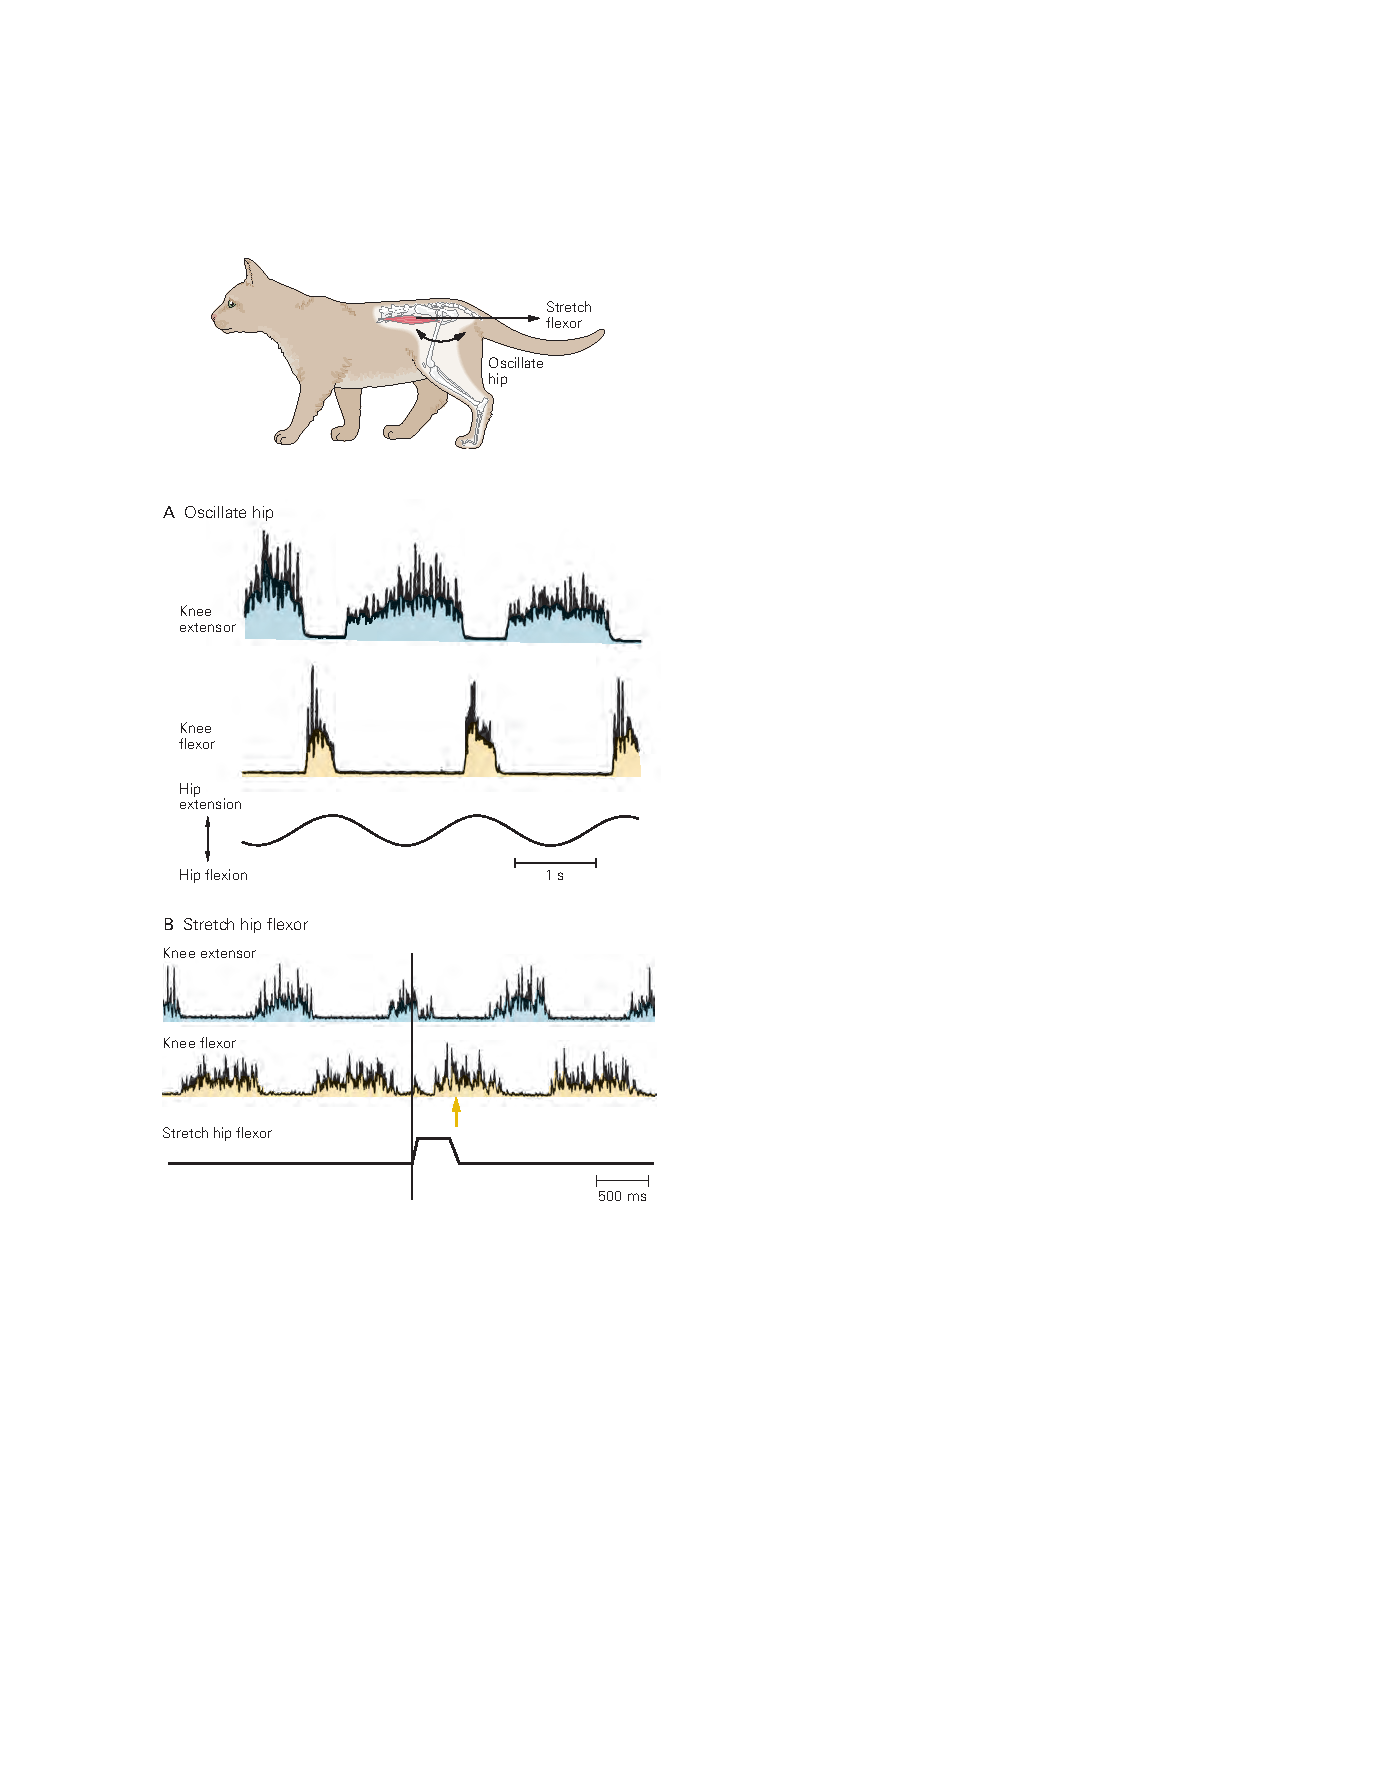
\includegraphics[width=0.5\linewidth]{chap33/fig_33_8}
	\caption{髋关节伸展启动了步行从站立阶段到摆动阶段的转变。 A. 在固定的去大脑猫中,髋关节周围的被动摆动运动启动并引起膝伸肌和屈肌运动神经元的虚拟运动模式。 屈肌肌电图 (EMG) 爆发对应于摆动阶段,并在髋关节伸展时产生。 (经许可改编自 Kriellaars 等人,1994 年。)B. 在行走的去大脑猫中,髋屈肌(髂腰肌)的拉伸抑制膝伸肌 EMG 活动,使膝屈肌活动更早开始。 膝屈肌记录中的箭头表示如果髋屈肌没有被拉伸,肌肉活动何时开始。 来自髋屈肌中肌梭的感觉纤维的激活是造成这种效果的原因。 (经许可改编自 Hiebert 等人,1996 年。)}
	\label{fig:33_8}
\end{figure}


来自高尔基肌腱器官和踝伸肌中肌梭的感觉纤维的激活会延长站立期,通常会延迟摆动期的开始,直到刺激结束(图 \ref{fig:33_9}A)。
来自两种类型感受器的感觉纤维在站立期间都很活跃,来自高尔基肌腱器官的信号强度与腿部承受的负荷密切相关。
高尔基体腱器官在身体静止时(第 \ref{chap:chap32} 章)对踝关节伸肌运动神经元有抑制作用,但在行走时有兴奋作用。
这种反射信号的逆转是由抑制性中间神经元通路的抑制以及运动过程中兴奋性通路的释放引起的。
在运动过程中这种反射逆转的功能性结果是,直到伸肌卸载并且这些肌肉施加的力很低时才开始摆动阶段,正如站立末尾附近高尔基肌腱器官活动减少所表明的那样。


\begin{figure}[htbp]
	\centering
	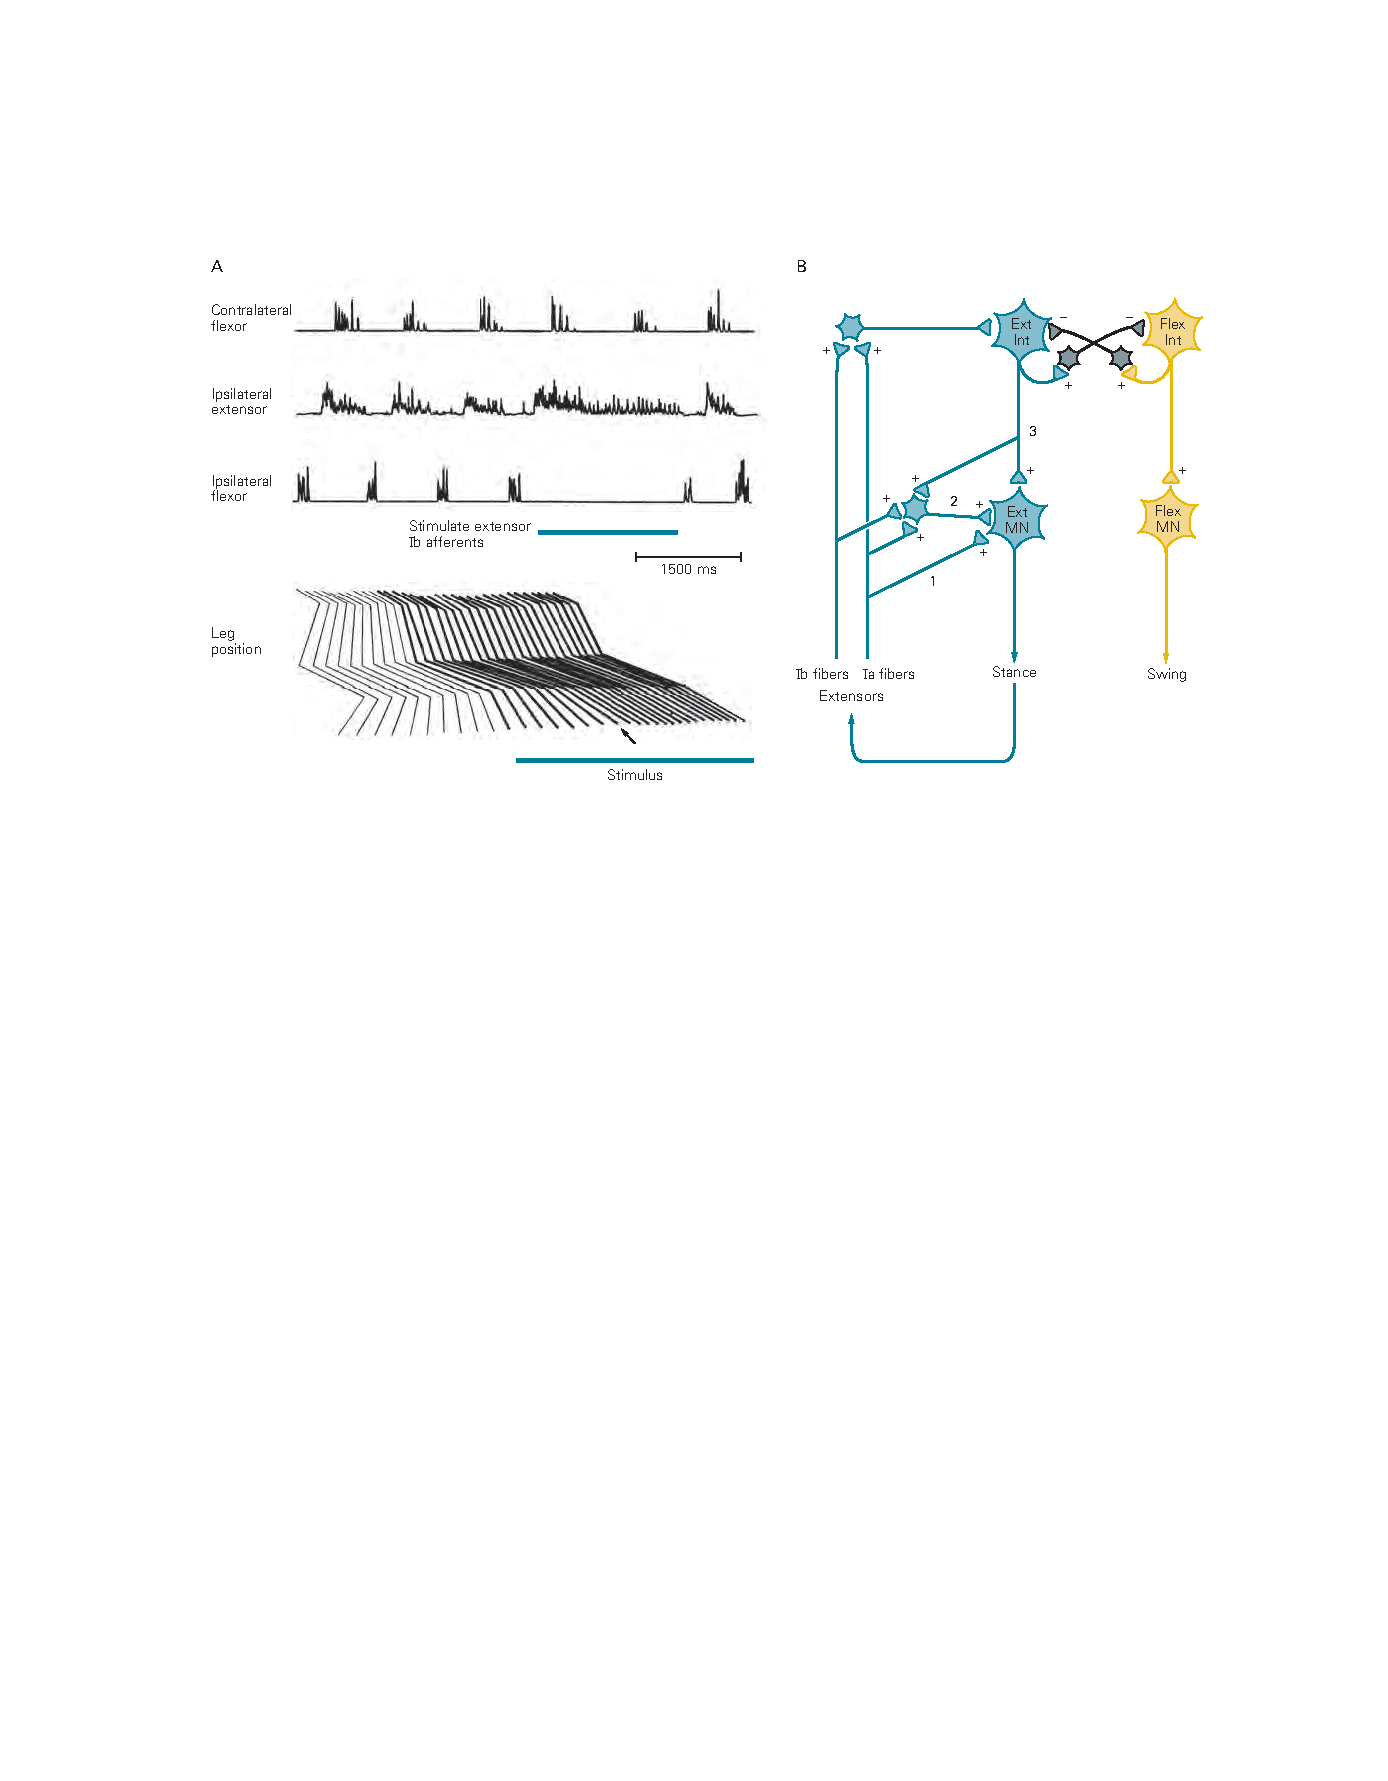
\includegraphics[width=0.9\linewidth]{chap33/fig_33_9}
	\caption{行走的摆动阶段由伸肌的感觉反馈启动。 A. 在去大脑猫中,来自踝伸肌的 I 组感觉纤维的电刺激抑制了同侧屈肌的肌电图爆发,并延长了行走期间同侧伸肌的爆发。 对侧屈肌活动的时间没有改变。 刺激来自踝关节伸肌的 I 组纤维可防止摆动期的启动,正如在刺激纤维时腿部的位置所见。 箭头显示如果踝伸肌传入神经未受到刺激,摆动期通常会发生的点。 (经许可改编自 Whelan、Hiebert 和 Pearson 1995。版权所有 © Springer-Verlag 1995。)B. 相互抑制的伸肌 (Ext) 和屈肌 (Flex) 中间神经元 (Int) 组构成传入通路中的节奏发生器 调节站立相。 来自伸肌的反馈增加了站立阶段伸肌运动神经元 (MN) 的活动水平,并在伸肌负荷时保持伸肌活动。 反馈通过三个兴奋性 (+) 通路传递:(1) 从 Ia 纤维到伸肌运动神经元的单突触连接; (2) 从 Ia 和 Ib 纤维到伸肌运动神经元的非突触连接; (3) 多突触兴奋通路,通过伸肌节律发生器起作用,以维持伸肌运动神经元在站立相中的活跃。}
	\label{fig:33_9}
\end{figure}


总之,来自踝关节伸肌和髋屈肌的本体感受信号协同工作,以促进从站立到摆动的阶段转变。
在站立后期,当肢体卸载时,随着来自高尔基肌腱器官的抑制信号减弱,它们对伸肌节律产生的影响减弱,同时髋关节周围的肌肉传入神经活动增加,促进屈肌活动 节奏的产生。


在步行过程中,至少有三种兴奋性通路将感觉信息从伸肌传递到伸肌运动神经元:来自初级肌梭(Ia 组传入)的单突触通路,来自初级肌梭和高尔基肌腱器官(Ia 和 Ib 组传入)的突触通路, 以及来自初级肌梭和高尔基肌腱器官的多突触通路,包括伸肌节律发生器中的中间神经元(图 \ref{fig:33_9}B)。
这些路径都有助于在脚踝卸载时从站立到摆动的阶段转变,并在脚踝加载时将伸肌保持在站立阶段。


除了调节从站立到摆动的转变外,来自肌梭和高尔基肌腱器官的本体感受信息对伸肌运动神经元爆发活动的产生有显着贡献。
减少猫的这种感觉输入会使伸肌活动水平降低一半以上;
在人类中,据估计高达 30\% 的踝关节伸肌运动神经元活动是由伸肌的反馈引起的。


\subsection{皮肤中的机械感受器允许行走以适应意外障碍}

皮肤中的机械感受器,包括一些伤害感受器,对行走时的 CPG 有很大的影响。
这些感受器的一项重要功能是检测障碍物并调整步进动作以避开障碍物。
一个经过充分研究的例子是猫对绊倒的纠正反应。


在摆动阶段对爪子的背部施加温和的机械刺激会产生屈肌运动神经元的兴奋和伸肌运动神经元的抑制,导致爪子快速弯曲远离刺激和抬高腿部以试图迈步 在对象上。
因为这种纠正反应很容易在脊髓猫身上观察到,所以它必须在很大程度上由完全包含在脊髓内的回路产生。


矫正反应的一个有趣特征是,只有在摆动阶段刺激爪子时,才会产生矫正屈曲运动。
在站立阶段施加相同的刺激会产生相反的反应——刺激伸肌,从而加强正在进行的伸肌活动。
这个伸肌动作是恰当的; 如果在站立阶段产生屈曲反射,动物可能会倒下,因为它是由肢体支撑的。
这是一个相位依赖反射逆转的例子。
相同的刺激可以在运动的一个阶段激发一组运动神经元,同时在另一阶段激活拮抗运动神经元。



\section{脊柱上结构负责步进的启动和自适应控制}

虽然运动的基本运动模式是在脊髓中产生的,但运动的启动、选择和规划需要激活脊髓上结构,包括脑干、基底神经节、小脑和大脑皮层。
步进的脊柱上调节提供了许多不能仅由脊髓回路介导的行为改变。
这些包括运动的自愿启动和速度调节;
姿势调节,包括重量支撑、平衡和肢间协调;
步态的预期修改的计划和执行,特别是视觉引导的修改。



\subsection{中脑核启动并维持运动和控制速度}

脊髓中的运动网络需要来自脊髓上区域的命令或启动信号来启动和维持它们的活动。
参与脊椎动物启动的主要神经元结构是中脑中称为中脑运动区 (MLR) 的区域。
MLR 最初是在猫身上发现的,它是位于楔形核内或周围的单一区域,就在下丘下方。
在静止动物的这个区域进行强直电刺激会增加姿势紧张,使动物站起来,然后开始行走。
随着刺激强度的增加,运动速度增加,交替步态切换为同步步态,例如疾驰或跳跃(图 \ref{fig:33_10})。


\begin{figure}[htbp]
	\centering
	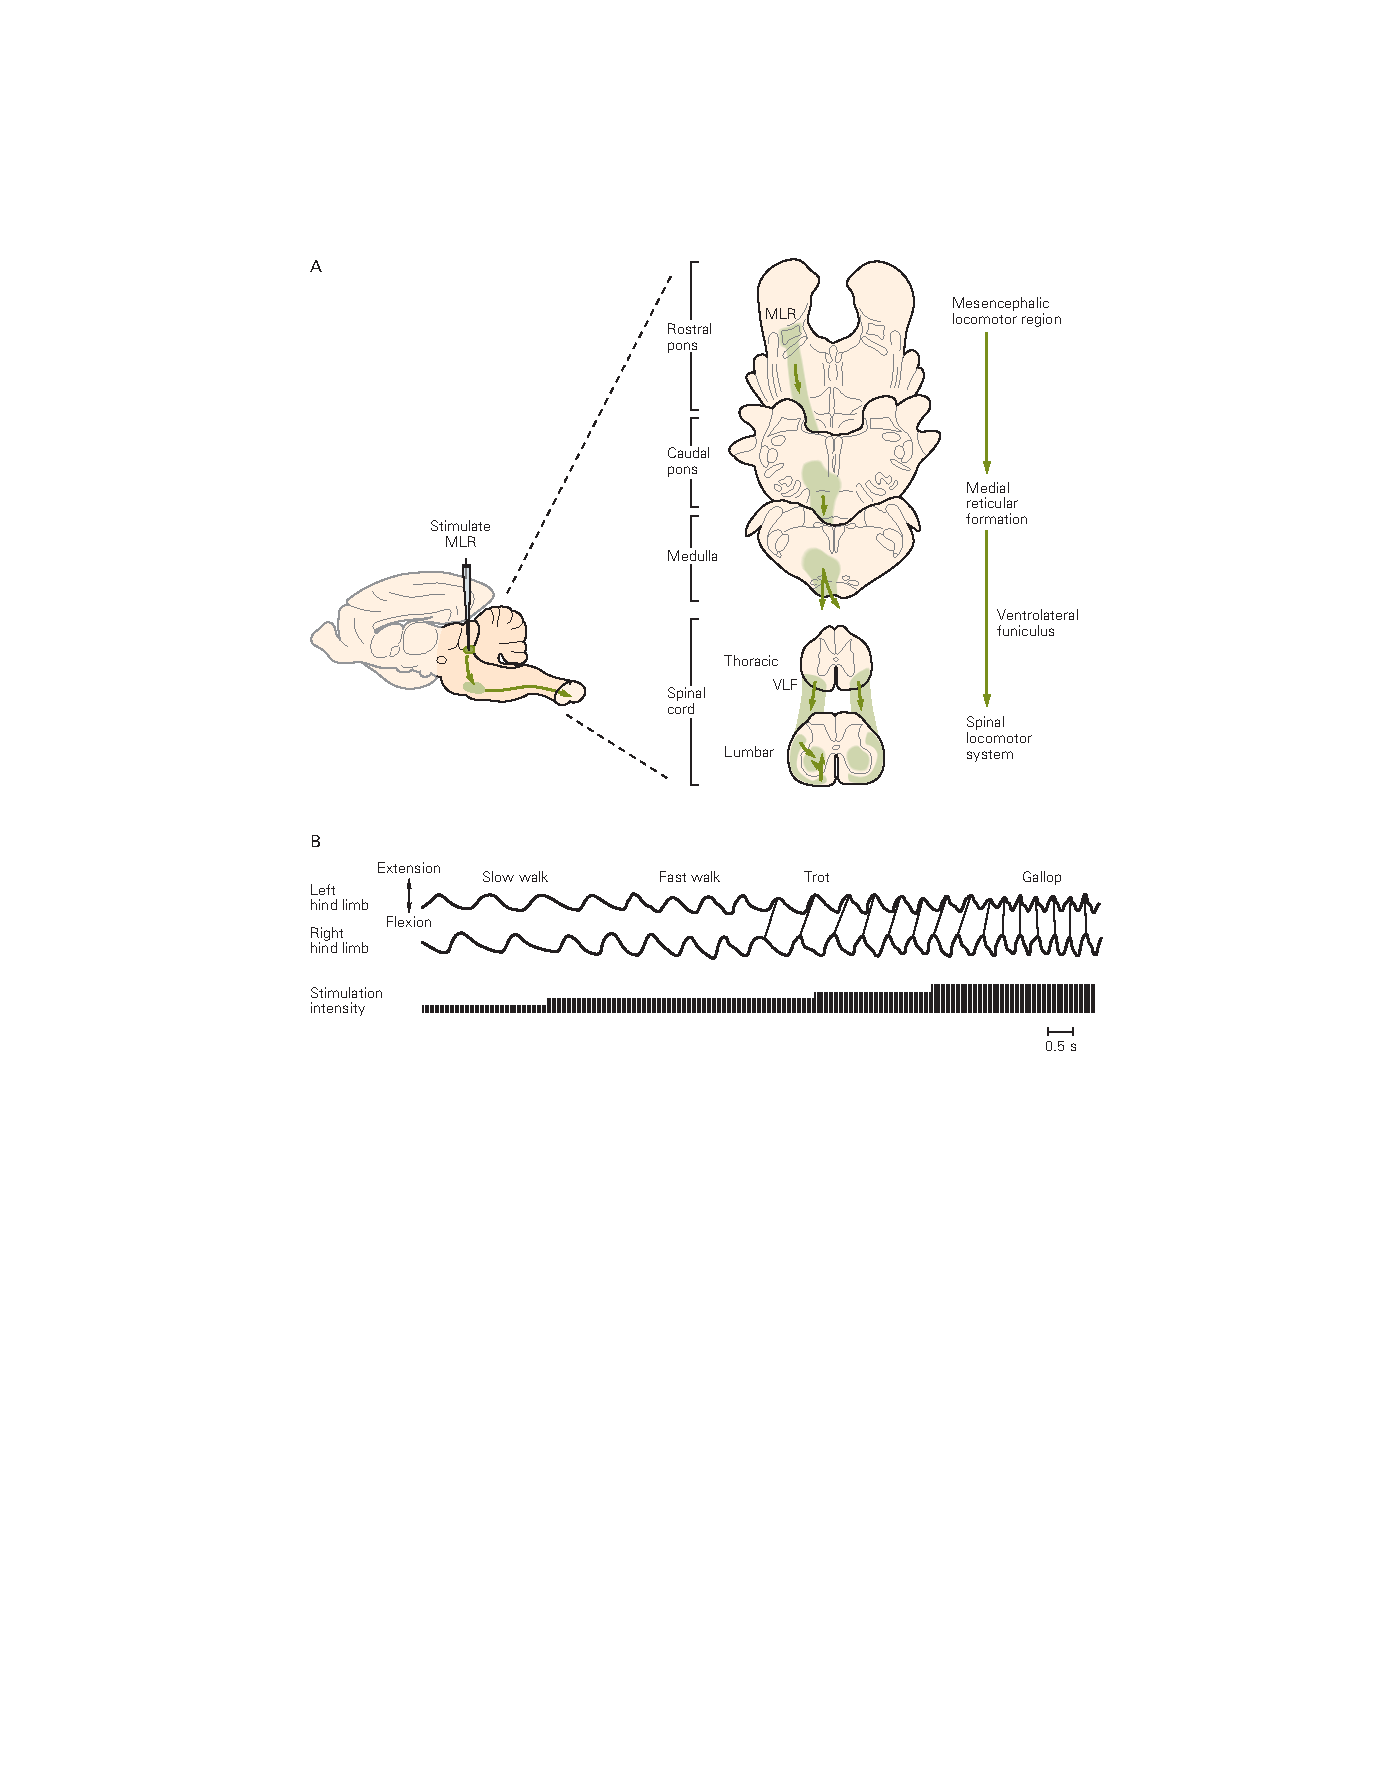
\includegraphics[width=0.7\linewidth]{chap33/fig_33_10}
	\caption{中脑运动区启动运动。 A. 猫中脑运动区 (MLR) 的电刺激通过激活内侧网状结构中的神经元启动运动,这些神经元的轴突在腹外侧索 (VLF) 中下降到脊髓运动系统。 B. 当在跑步机上行走的去大脑猫的 MLR 电刺激强度逐渐增加时,步态和步速从慢走变为小跑,最后变为疾驰。 随着猫从小跑发展到疾驰,后肢从交替活动转变为同相活动。 (改编自 Shik 等人,1966 年。)}
	\label{fig:33_10}
\end{figure}

后来的电刺激研究证实了 MLR 在所有脊椎动物中的存在,表明 MLR 从最古老的脊椎动物到人类在进化上是保守的。
这些研究指出了两个中脑结构作为 MLR 的一部分(图 \ref{fig:33_11}A):楔形核 (CNF) 和位于腹侧的脚桥核 (PPN)(图 \ref{fig:33_11}A)。
这两个细胞核的不同之处在于它们包含的神经元类型。


\begin{figure}[htbp]
	\centering
	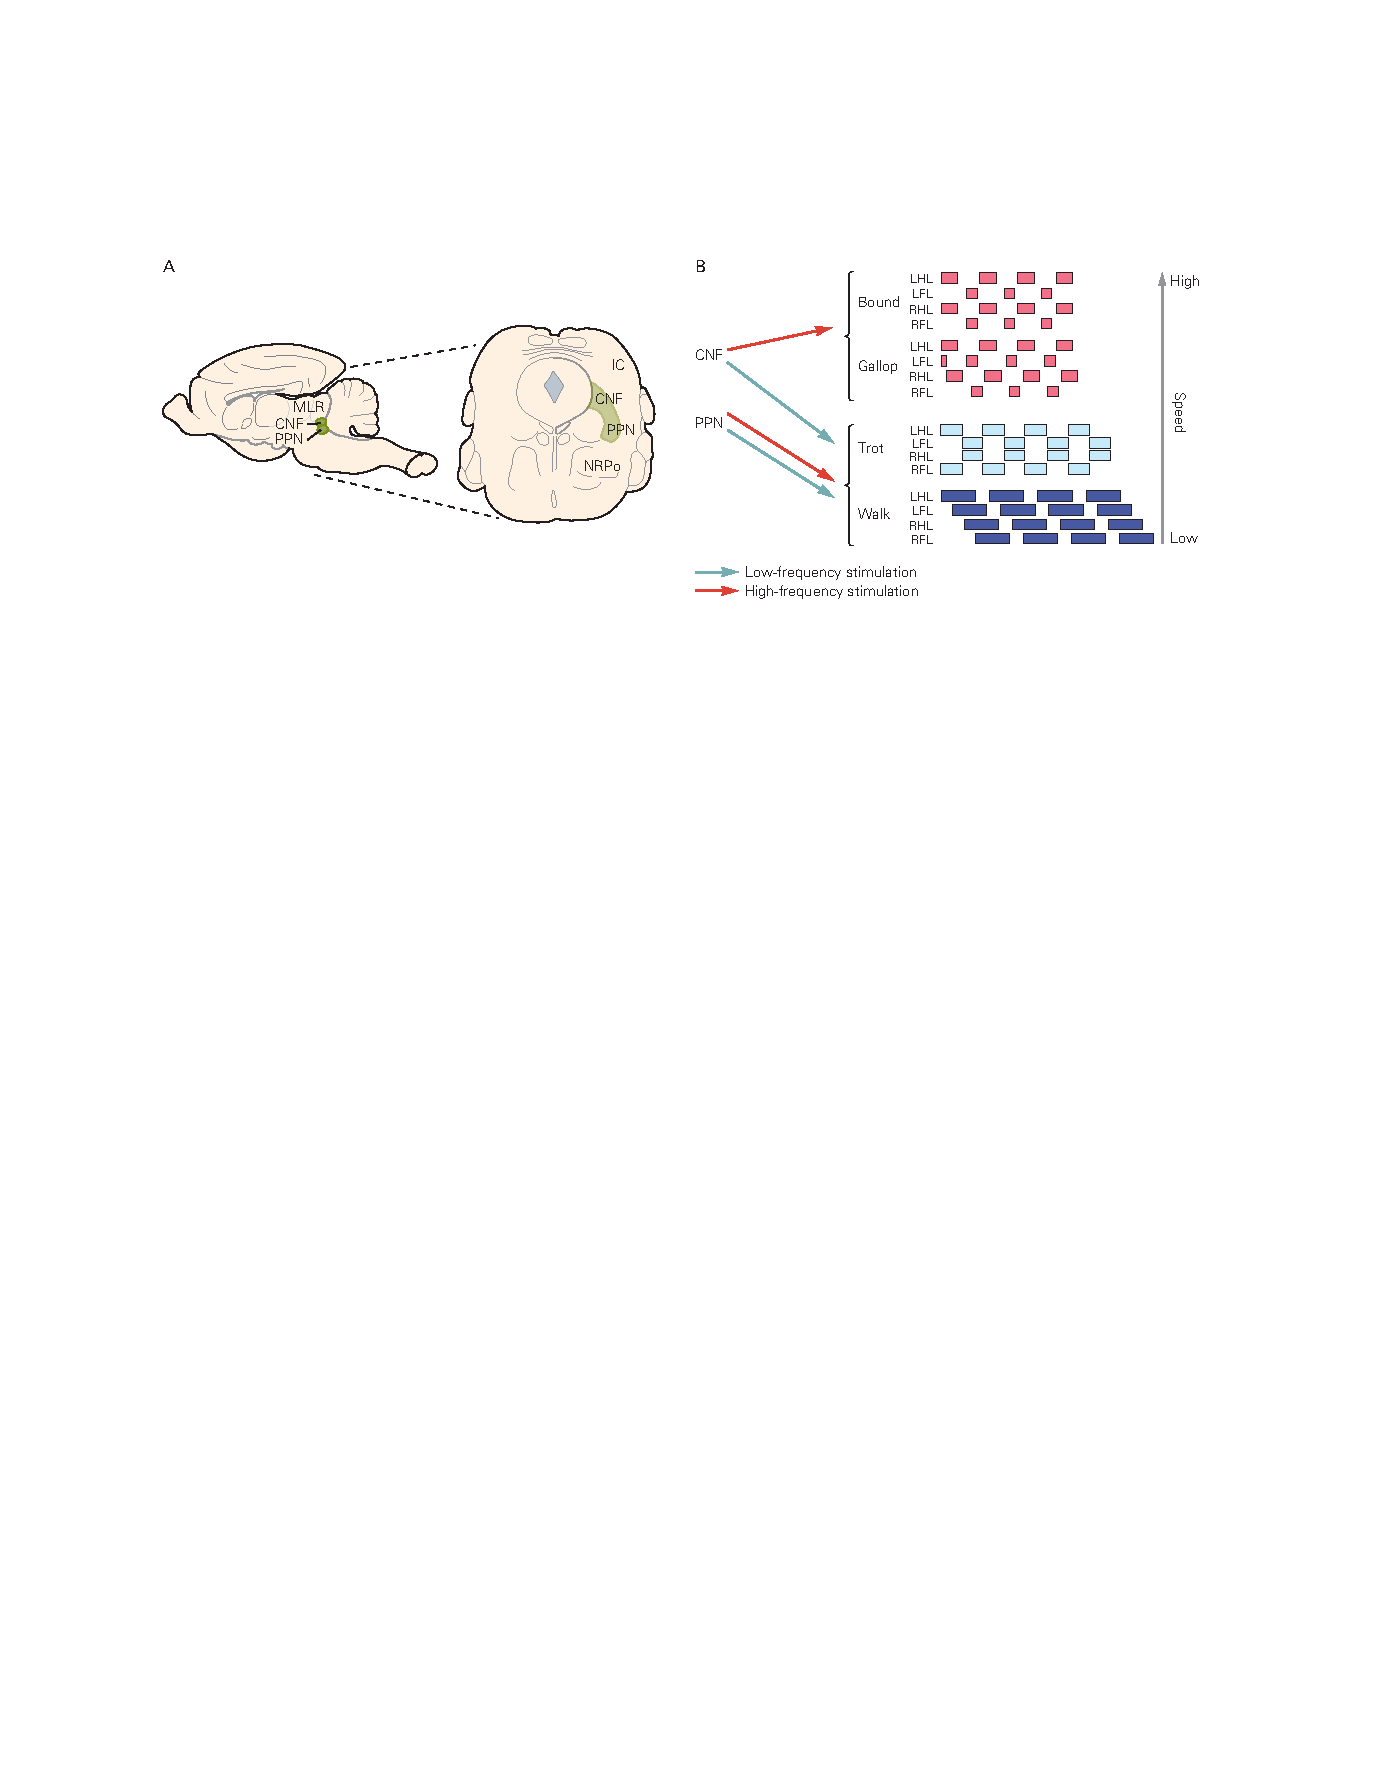
\includegraphics[width=0.9\linewidth]{chap33/fig_33_11}
	\caption{中脑运动区域由双中脑谷氨酸能核组成,可控制运动的启动、速度和步态调节以及运动的上下文相关选择。 A. 左图:小鼠中脑中脑运动区 (MLR) 的定位部位。 右图:横切面显示 MLR 由中脑的楔形核 (CNF) 和桥足核 (PPN) 组成,位于大脑导水管外侧,背侧为网状脑桥口核 (NRPo)。 谷氨酸能神经元、氨基丁酸能神经元和胆碱能神经元混合在 CNF 和 PPN 中。 (缩写:IC,下丘)。 B. 光刺激 CNF 或 PPN 中的谷氨酸能细胞对小鼠的影响,这些细胞已经转染了光敏通道,通道视紫红质 2。PPN 中的低频和高频刺激只会导致交替的步态——步行和小跑。 CNF 中的低频模拟同样只会导致缓慢的探索性运动,而高频刺激会引起与逃逸运动相对应的同步步态疾驰和跳跃。 不同类型的步态显示为从低速到高速运动的理想化图表。 实心方框代表站立阶段; 打开摆动阶段的空间。 步行的特点是同时由三只或四只脚支撑。 小跑的特点是前肢和后肢对角线同时活动。 疾驰的特点是前肢移动时略有异相,而后肢几乎同相。 Bound的特点是后肢和前肢同时运动,前肢和后肢不同步。 (缩写:LFL,左前肢;LHL,左后肢;RFL,右前肢;RHL,右后肢。)(改编自 Caggiano 等人 2018 年的数据。)}
	\label{fig:33_11}
\end{figure}

CNF 中的远程投射神经元是兴奋性的,并使用谷氨酸作为它们的神经递质,而 PPN 中的神经元既是谷氨酸能又是胆碱能的。
在两个细胞核中,兴奋性神经元与局部 GABAergic 中间神经元混合在一起。
然而,电刺激无法确定哪个细胞核或哪种类型的神经元参与了运动和速度控制的启动。
然而,使用神经递质特异性 CNF 和 PPN 神经元的选择性激活和失活表明这两个核在运动的速度控制和步态选择中发挥特定作用(图 \ref{fig:33_11}B)。
PPN 和 CNF 中的谷氨酸能神经元足以支持慢速交替运动,例如步行和小跑,而 CNF 中的谷氨酸能神经元是高速运动所必需的,例如疾驰和跳跃,逃逸运动的特征。
这些步态的表达取决于刺激频率,可能反映了完整动物中发射频率的影响。


胆碱能 PPN 神经元在运动中的作用尚不清楚。 在哺乳动物中,它们似乎在维持运动方面没有很强的作用。


谷氨酸能 CNF 和 PPN 神经元在运动控制中的这些作用也可能反映在不同的输入中。
PPN 神经元从基底神经节接收强输入,特别是黑质网状部、苍白球内部和底丘脑核,以及来自感觉运动和额叶皮层的输入。
此外,PPN 从中脑和脑干中的许多核团接收感觉运动信息。
因此,细胞核可以作为整合来自许多大脑结构的信息的枢纽,可能导致释放较慢的探索性运动。
相比之下,CNF 中神经元的输入受到更多限制,主要来自可能参与逃避反应的结构。
因此,MLR 由两个区域组成,这两个区域共同作用以选择依赖于上下文的运动行为。


另一个在受到刺激时引起运动的大脑区域是丘脑底(或间脑)运动区(与丘脑底核区分开来)。
该区域包括背侧和外侧下丘脑中的细胞核,这些细胞核参与各种稳态功能,例如调节进食。
这些区域的神经元投射到网状结构中的神经元并绕过 PPN 和 CNF,这表明启动运动的平行路径可能是由寻找食物的需要驱动的。


\subsection{启动脑干神经元运动项目的中脑核}

来自 CNF 和 PPN 的兴奋信号通过脑干网状结构中的神经元间接传递到脊髓,从而为脊髓中的运动网络提供最终命令信号。
这些神经元的身份只是部分已知。
一般而言,涉及两个递质定义的途径:谷氨酸能和血清素能。


谷氨酸能运动通路可能在脑干网状结构中有多个起源,形成平行的下行通路。
它们通过节间(脊髓本体)谷氨酸能中间神经元链直接或间接投射到脊髓中的运动神经元(图 \ref{fig:33_10}A)。
网状脊髓神经元也参与调节动物运动所需的姿势活动(见后面的讨论)。


哺乳动物中存在 5-羟色胺能运动通路的证据仅限于大鼠实验,这些实验表明 5-羟色胺能神经元参与脑干尾部。
从脑干到脊髓的最终命令信号激活脊髓运动网络、维持其活动并允许表达不同步态的机制尚不清楚。


运动的偶发性表明启动信号可能由停止命令补充,以允许运动突然停止。
此类信号已在非洲爪蟾蝌蚪中发现,其中头部与障碍物接触会激活 GABAergic 下行通路,从而立即终止游泳。
同样,在去大脑的猫中,延髓和尾部桥脑网状结构的强直电刺激会导致一般的运动抑制。
对小鼠的研究已经确定了网状结构中 V2a 神经元的受限特遣队,这些神经元介导了正在进行的运动活动的立即停滞。
这种“V2a 停止神经元”通过下行投射向腹侧腰椎脊髓中抑制节律生成的抑制性中间神经元发送行为相关的停止信号。
类似的停止信号会阻止七鳃鳗游泳。


\subsection{脑干核团在运动过程中调节姿势}

运动控制的一个重要方面是姿势的调节。
这个通用术语包含几种类型的行为,包括运动叠加的姿势支持的产生、平衡的控制、四足动物肢间协调的调节,以及适应斜坡上或在斜坡上运动所需的肌肉紧张度的改变 转动。
此外,姿势的预期变化先于自愿步态修改的变化,姿势的补偿性变化遵循意想不到的扰动。
这些功能主要由起源于脑干的两个下行系统提供支持:起源于前庭外侧核 (LVN) 的前庭脊髓束 (VST) 和起源于桥延髓网状结构 (PMRF) 的网状脊髓束 (RST)。
这两种途径在系统发育上都很古老,并且存在于所有脊椎动物中。


LVN、PMRF 或其在脊髓中的下行轴突的损伤导致体重支撑和平衡控制的丧失,表现为蹲伏步态和后躯向一侧或另一侧摇摆。
这些细胞核的损伤也会导致前肢和后肢之间的肢间协调发生巨大变化。
同样,对脑桥和延髓的强直电刺激或化学刺激可调节四肢肌肉紧张的水平,并可促进或抑制运动,具体取决于刺激的确切部位(图 \ref{fig:33_12})。


\begin{figure}[htbp]
	\centering
	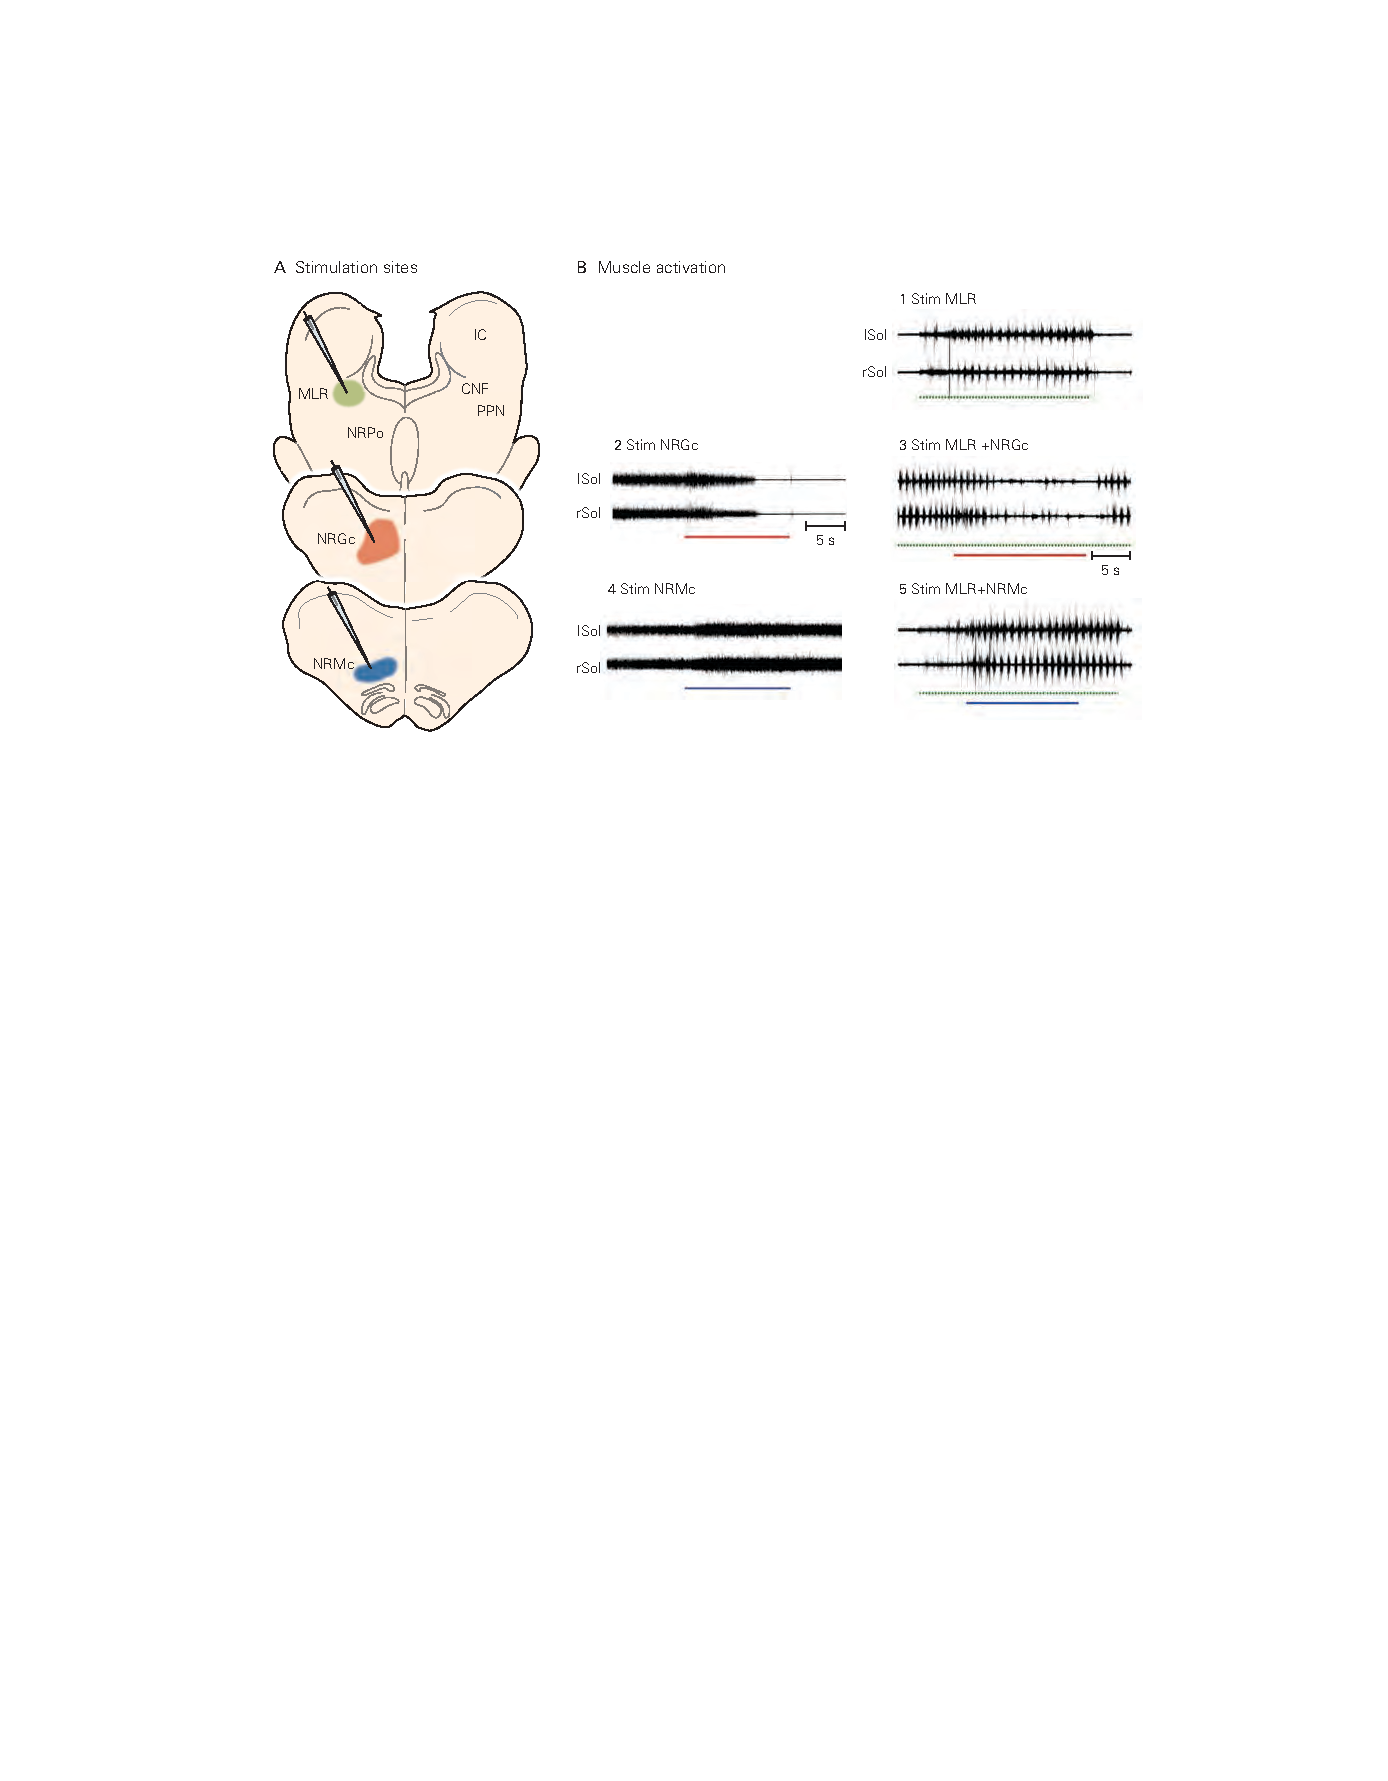
\includegraphics[width=0.8\linewidth]{chap33/fig_33_12}
	\caption{运动活动通过姿势音调的水平进行修改。 (经许可改编自 Takakusaki 等人,2016 年。)A. 猫脑干在三个不同的头尾水平的横切面。 彩色区域表示 B 部分所示试验期间受刺激的区域。(缩写:CNF,楔形核;IC,下丘;MLR,中脑运动区;NRPo,脑桥口部网状核;NRGc,巨细胞网状核;NRMc,网状核 magnocellularis;PPN,脚桥核。) B. 刺激脑干不同区域的效果,如 A 部分所示,对去大脑猫。 1. 刺激 MLR (CNF/PPN)(绿色条)在左右后肢比目鱼肌 (Sol) 中产生有节奏的激活。 2. 强直刺激髓质中的 NRGc(红色条)会导致伸肌肌张力下降。 3. 在 CNF 诱导的运动过程中刺激 NRGc 会降低肌肉张力,从而抑制运动。 4. 强直刺激腹侧髓质中的 NRMc(蓝色条)会增加肌肉张力。 5. 在 MLR 刺激期间刺激 NRMc 导致运动活力增加。}
	\label{fig:33_12}
\end{figure}


VST 和 RST 中的活动以及源自红核的红核脊髓束中的活动也会阶段性地改变每个步骤中的肌肉紧张水平。
这三种结构中任何一种的弱电刺激都会产生运动活动的相位依赖性调制。
用短刺激序列短暂激活这些通路会在肌肉爆发的幅度上产生瞬时变化,但很少在步进周期的时间上产生任何变化。
LVN 的激活主要增强同侧伸肌在站立期自然活动期间的反应。
相比之下,刺激红核通常会使对侧屈肌的活动短暂增加,同样是在摆动期的自然活动期间。


PMRF 的刺激会产生更复杂和更广泛的反应,这些反应可能会以协调的模式改变所有四肢在摆动阶段屈肌和站立阶段伸肌的活动(图\ref{fig:33_13})。
在屈肌中,PMRF 刺激通常会促进活动,但在伸肌中,活动可能会根据受刺激的确切部位而得到促进或抑制。
这种反应的相位依赖性被认为是由脊髓 CPG 中中间神经元的激活介导的。
以更高的强度或更长的序列刺激这三个结构,可能会改变步进周期的时间以及 EMG 活动的幅度。


\begin{figure}[htbp]
	\centering
	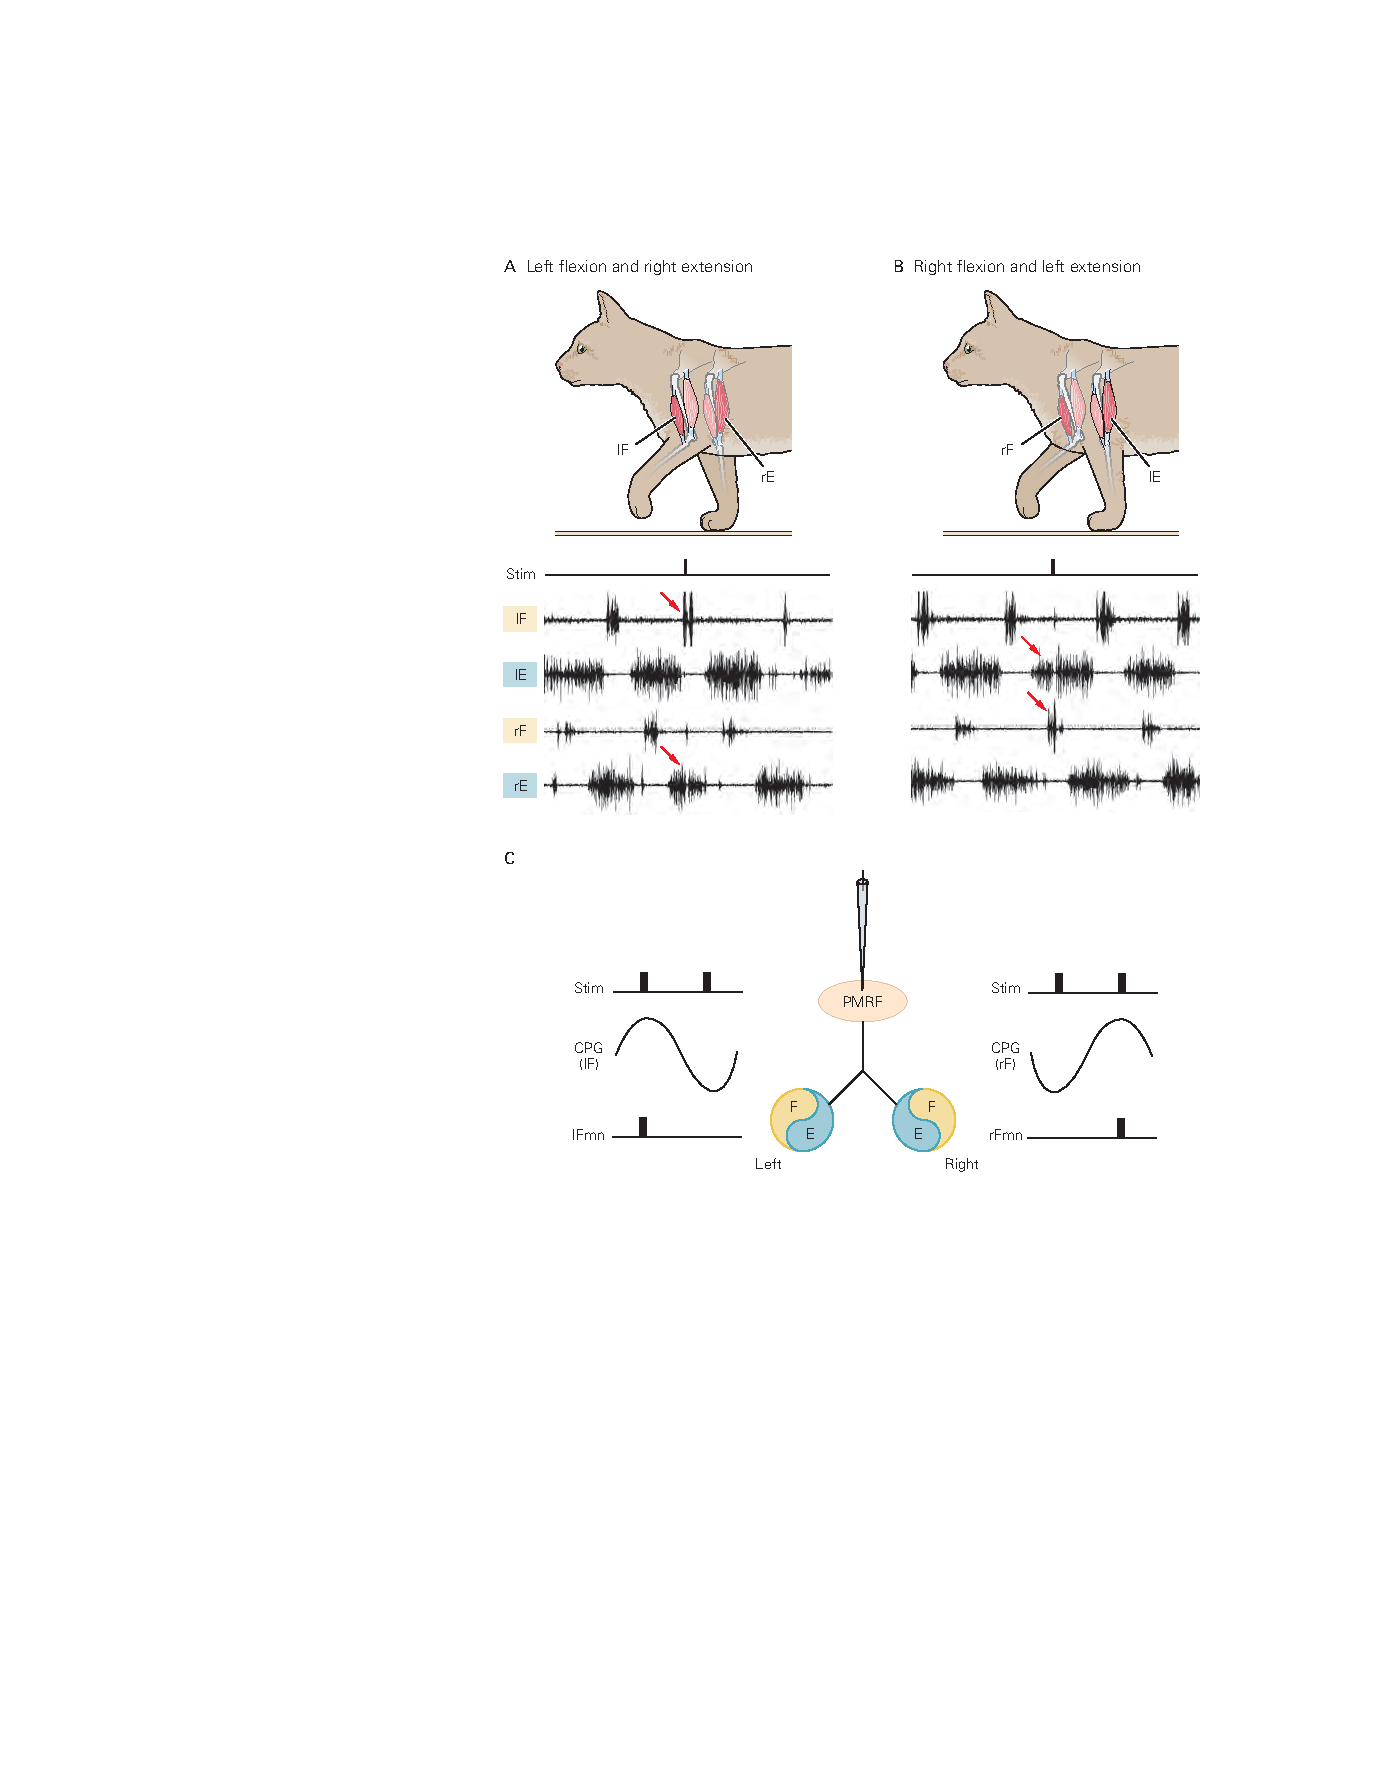
\includegraphics[width=0.7\linewidth]{chap33/fig_33_13}
	\caption{桥延髓网状结构 (PMRF) 的微刺激会在屈肌和伸肌中产生相位依赖性反应。 (来自 T. Drew 的数据。)A. 在左肢摆动阶段刺激左 PMRF 会导致左屈肌 (lF) 肌电图活动短暂增加,同时右伸肌活动减少 (rE)(红色箭头)。 左伸肌 (lE) 或右屈肌 (rF) 几乎没有刺激诱发的活动,它们在踏步周期的这个阶段处于非活动状态。 B. 在右肢摆动阶段,在 PMRF 的同一位置进行刺激会产生相反的反应。 C. 响应的相位依赖性可能由中间神经元兴奋性水平的周期性决定,中间神经元是运动中央模式发生器 (CPG) 的一部分。 响应由运动 CPG 的屈肌 (F) 和伸肌 (E) 部分的活动门控。 当第一个刺激到达时,左侧 CPG (lF) 中的屈肌中间神经元处于活动状态,而右侧 CPG (rF) 中的屈肌中间神经元处于非活动状态。 因此,刺激仅在左屈肌运动神经元 (lFmn) 中产生反应。 当第二次刺激到达时,右侧 CPG (rF) 中的屈肌中间神经元处于活动状态,而左侧的屈肌中间神经元处于非活动状态,因此,刺激仅在右侧的屈肌运动神经元 (rFmn) 中引起反应。}
	\label{fig:33_13}
\end{figure}


在运动过程中,LVN、PMRF 和红核内的神经元以步进周期的频率进行相位调制。
LVN 中的神经元通常与同侧伸肌同步激活,而红核中的神经元通常在对侧摆动期激活。
PMRF 中的神经元具有更复杂的活动周期,并且可能与同侧或对侧屈肌或伸肌相关地放电。


脑干结构也有助于运动过程中更复杂的活动。
例如,红核有助于精确修改步态所需的肌肉活动的复杂修改(见下文)。
以互补的方式,PMRF 对多个肢体的广泛影响使其能够产生伴随步态修改的姿势活动的协调变化。
从运动皮层到 PMRF 的强连接确保了步态修改和姿势活动之间的协调,其方式与离散的自愿运动相同(第 \ref{chap:chap34} 章)。
PMRF 还有助于由于扰动而发生的姿势补偿性变化。
在这种情况下,它形成了脊髓-球-脊髓反射的一部分,这种反射有助于广泛的姿势反应,这些姿势反应遵循由突然扰动激活的即时脊髓反射。



\section{视觉引导运动涉及运动皮层}

行走通常由视觉引导,而运动皮层对于视觉引导的运动非常重要,尤其是当必须修改步态以确保精确控制肢体轨迹和足部放置时。
在哺乳动物中,运动皮层的损伤不会阻止动物在光滑的地板上行走,但会严重损害“精确运动”,这需要高度的视觉运动协调能力,例如在水平梯子的横档上行走,跨过 一系列障碍,并跨过放置在跑步机皮带上的单个物体。


在受过训练以跨过连接到移动跑步机带上的障碍物的完整猫身上进行的实验表明,精确运动与运动皮层中众多神经元活动的显着调节有关(图 \ref{fig:33_14})。
运动皮层中的其他神经元表现出更加离散的活动模式,并在摆动期的不同部分依次被激活。
这些皮层神经元的活动与产生步态修改所需的修改肌肉活动的周期相关,其方式与到达期间发生的方式类似(见图 34-21)。
这种神经元亚群可能有助于改变产生肢体轨迹灵活变化所需的协同肌肉群的活动。


\begin{figure}[htbp]
	\centering
	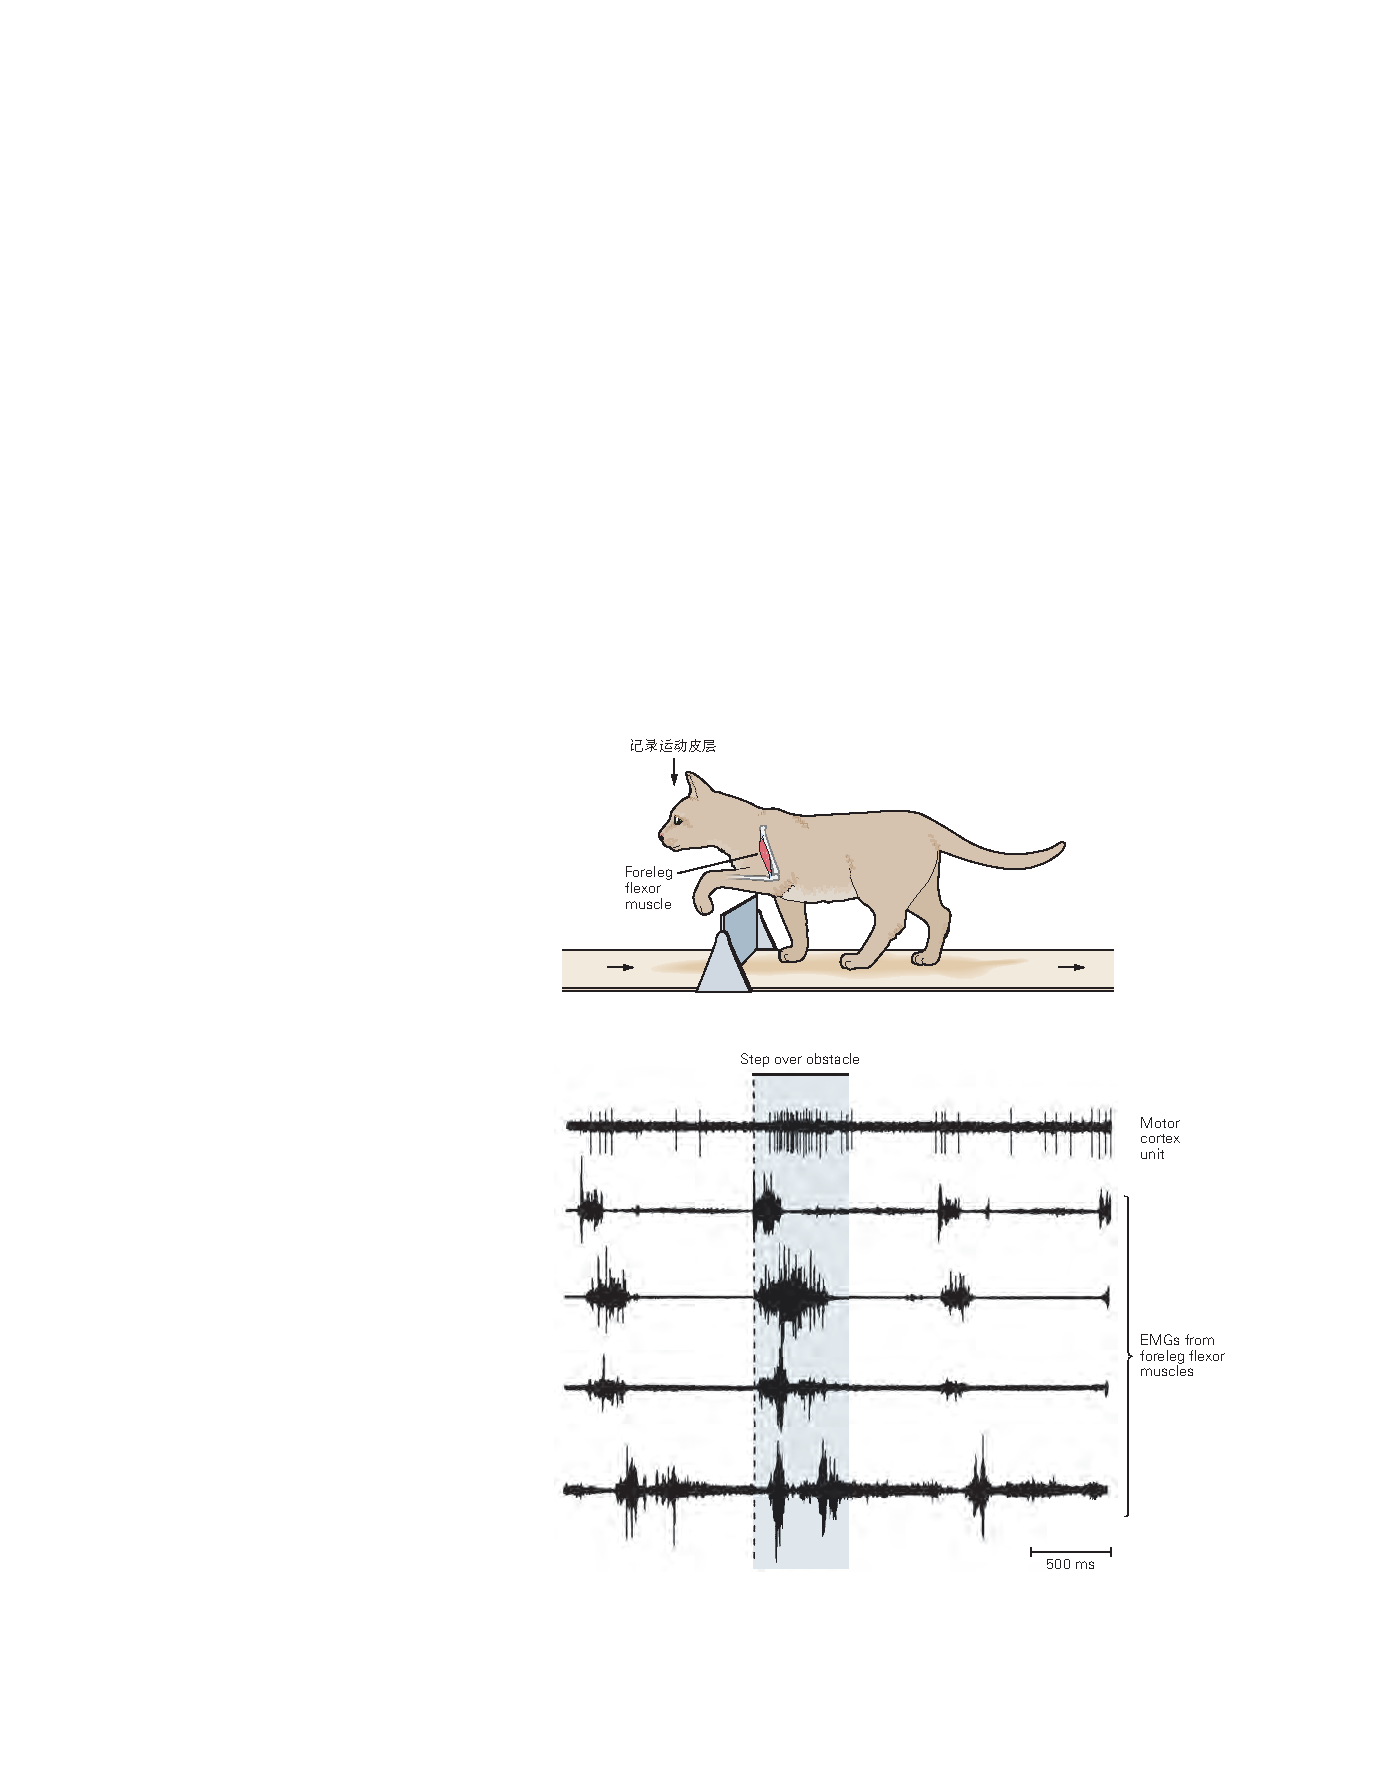
\includegraphics[width=0.75\linewidth]{chap33/fig_33_14}
	\caption{运动皮层响应视觉输入调整步进运动。 当一只猫跨过固定在跑步机上的可见物体时,运动皮层中的神经元会增加活动。 如肌电图 (EMG) 所示,皮质活动的增加与前腿肌肉活动的增强有关。 (经许可改编自 Drew 1988。)}
	\label{fig:33_14}
\end{figure}


许多这些皮层神经元直接投射到脊髓(皮质脊髓神经元),因此可以调节脊髓中间神经元的活动,包括 CPG 内的神经元,从而使运动活动的时间和幅度适应特定的运动任务。
应用于正常步行猫的运动皮层或皮质脊髓束的简短电刺激序列以相位依赖的方式在对侧肢体中产生瞬态反应,类似于各种脑干结构中的活动产生的反应。
然而,与用脑干结构观察到的情况相反,增加应用于运动皮层的刺激序列的持续时间经常导致运动节律的重置,其特征是正在进行的步循环中断和新的步循环的开始 步骤循环。
这表明在哺乳动物中,皮质脊髓束有特权访问 CPG 的节律发生器。


\section{运动规划涉及后顶叶皮层}

当人类和动物在他们的道路上接近障碍物时,他们必须调整他们的行走方式以绕过障碍物或跨过障碍物。
这些调整的计划在达到障碍之前的两到三个步骤开始。
最近的实验表明,后顶叶皮层 (PPC) 特别参与规划步态修改。
该区域的病变会导致行走的猫在接近障碍物时错放其爪子的位置,并增加一条或多条腿在跨过障碍物时接触障碍物的可能性。


与在运动皮层中观察到的情况相反,PPC 中的记录显示许多神经元在跨过障碍物之前增加了它们的活动。
此外,无论哪条腿先跨过障碍物,PPC 中的许多细胞都以类似方式放电(图 \ref{fig:33_15}A、B)。
这些细胞可以提供身体相对于环境中物体的位置的估计(图 \ref{fig:33_15}B),允许动物在接近障碍物时改变步态。
PPC 与通常被认为参与运动规划的其他皮质和皮质下结构相互作用的方式尚不清楚。
然而,最近的研究表明,前运动皮层也对规划视觉引导的步态修改做出了重要贡献(图 \ref{fig:33_15}C),并且可能涉及全局信号的转换,该信号提供有关障碍物位置的信息到运动所需的基于肌肉的信号。
跨越障碍的步骤的执行。


\begin{figure}[htbp]
	\centering
	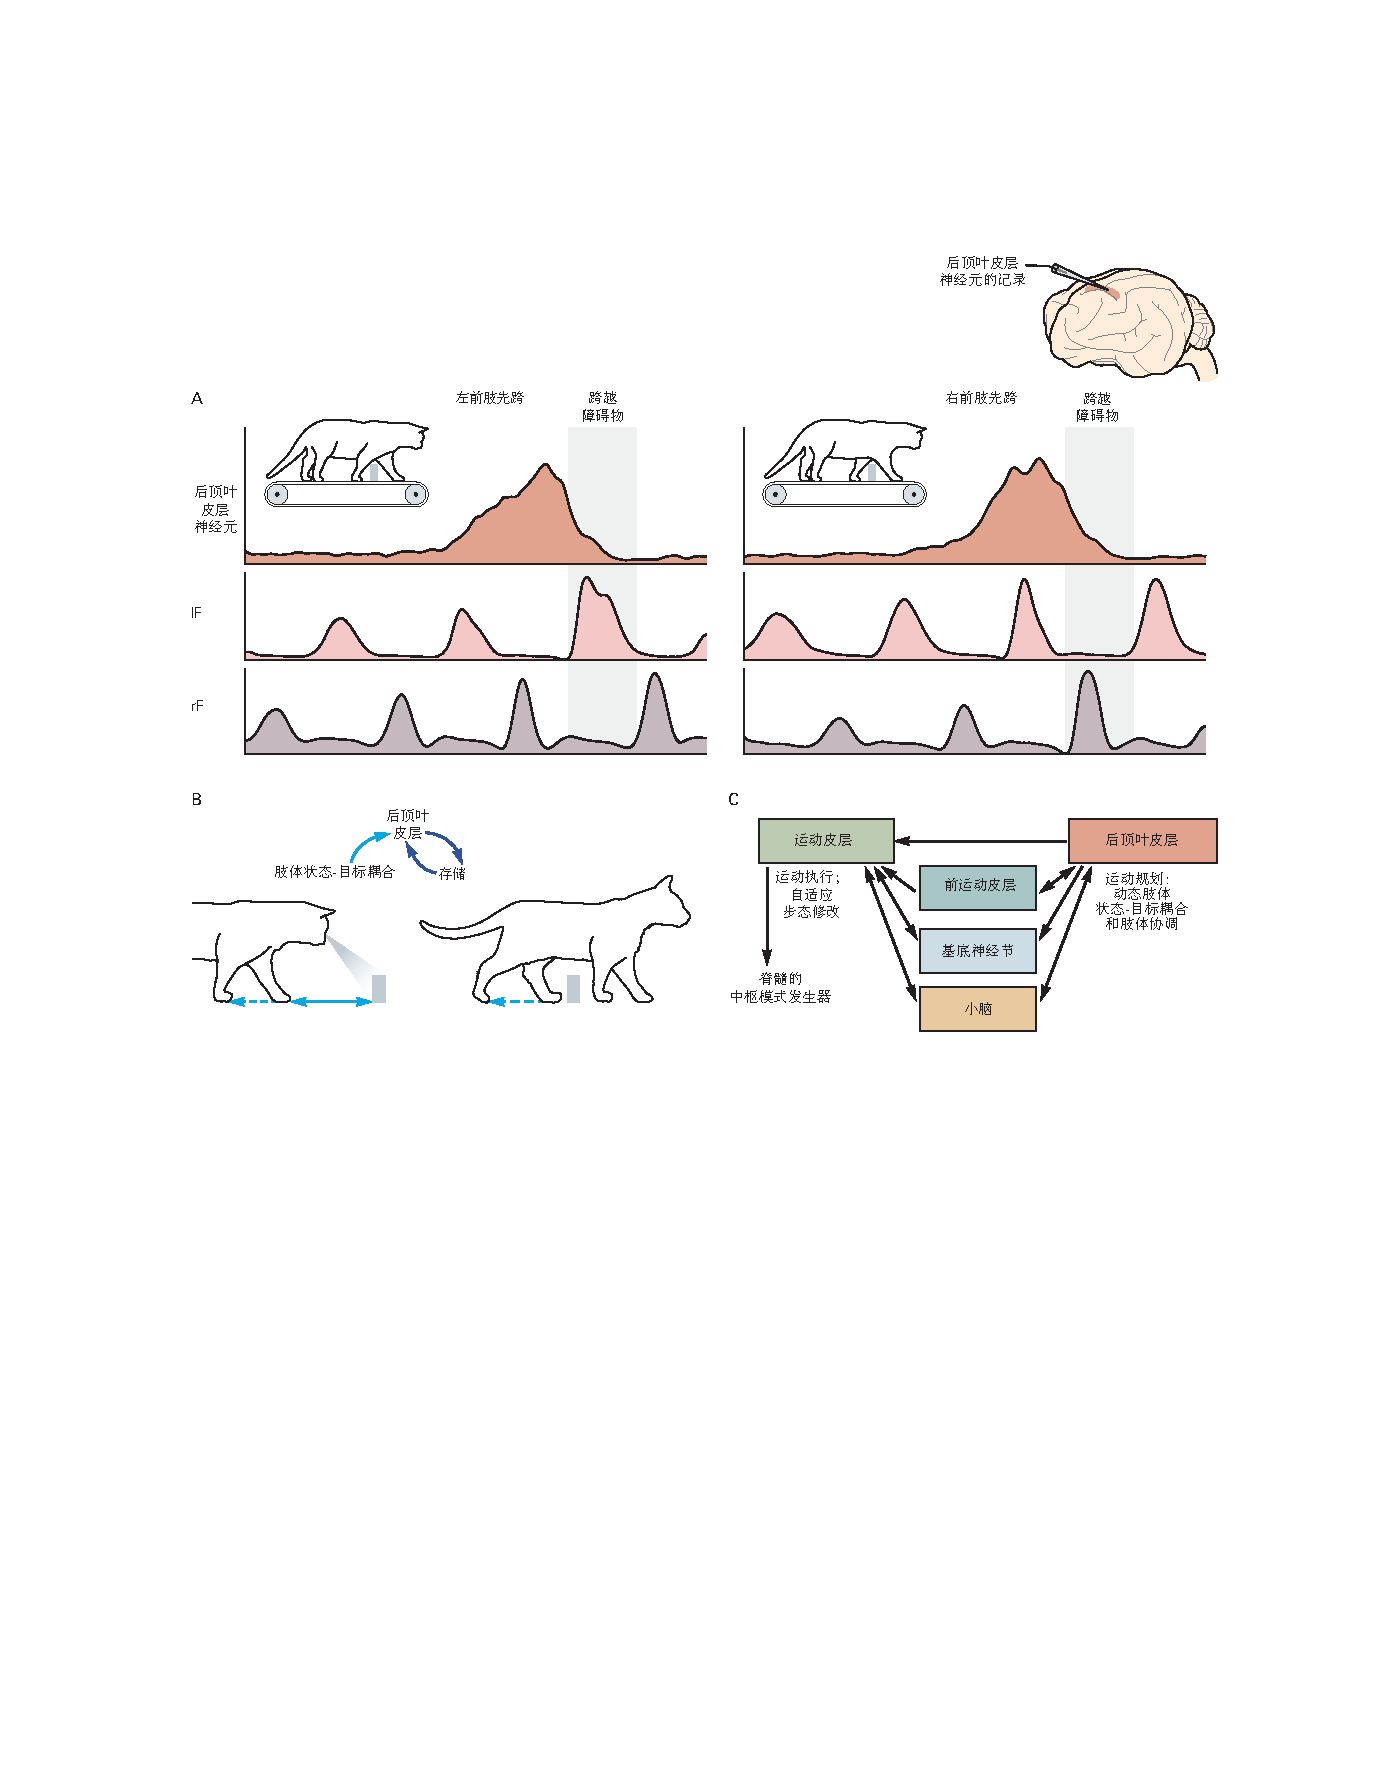
\includegraphics[width=0.95\linewidth]{chap33/fig_33_15}
	\caption{后顶叶皮层 (PPC) 中的神经元参与规划自愿步态修改。 A. 当左前肢或右前肢首先跨过障碍物时,右侧皮层中 PPC 神经元的活动。 在每种情况下,PPC 中的电池都会在越过障碍物之前提前两到三步放电。 B. 观察到 PPC 神经元的放电与第一个跨过障碍物的肢体无关,这表明 PPC 在运动规划中具有全局功能。 在一般方案中,PPC 神经元参与估计物体相对于身体的相对位置(肢体状态 - 物体耦合 [双箭头])和 PPC 中的存储信息以供以后检索。 C. PPC 在规划步态修改时并不单独行动。 它是皮层和皮层下网络的一部分,包括运动前皮层、基底神经节和小脑等结构。 这些结构中的每一个之间以及它们中的每一个与运动皮层之间都存在连接,运动皮层负责执行步态修改。 (缩写:CPG,中央模式发生器。)(经许可改编自 Drew 和 Marigold 2015。)}
	\label{fig:33_15}
\end{figure}


有关障碍物大小和位置的视觉信息也存储在工作记忆中,这是一种短期记忆形式(第 \ref{chap:chap52} 章)。
此信息用于确保后肢的步态修改与前肢的步态修改相协调,并且是必要的,因为当后肢跨过障碍物时,障碍物已不在视野内。
这种形式的工作记忆背后的神经生物学机制仍有待确定,但记忆的持久性似乎至少部分取决于 PPC 中的神经元系统。
随着双侧损伤或内侧 PPC 冷却,记忆完全消失(图 \ref{fig:33_16}A)。
补充这一观察结果是,PPC 中某些神经元的活动在跨过障碍物的过程中以及在动物跨过障碍物的整个过程中升高(图 \ref{fig:33_16}B)。
此活动可以代表障碍物关键特征(例如高度)的工作记忆。


\begin{figure}[htbp]
	\centering
	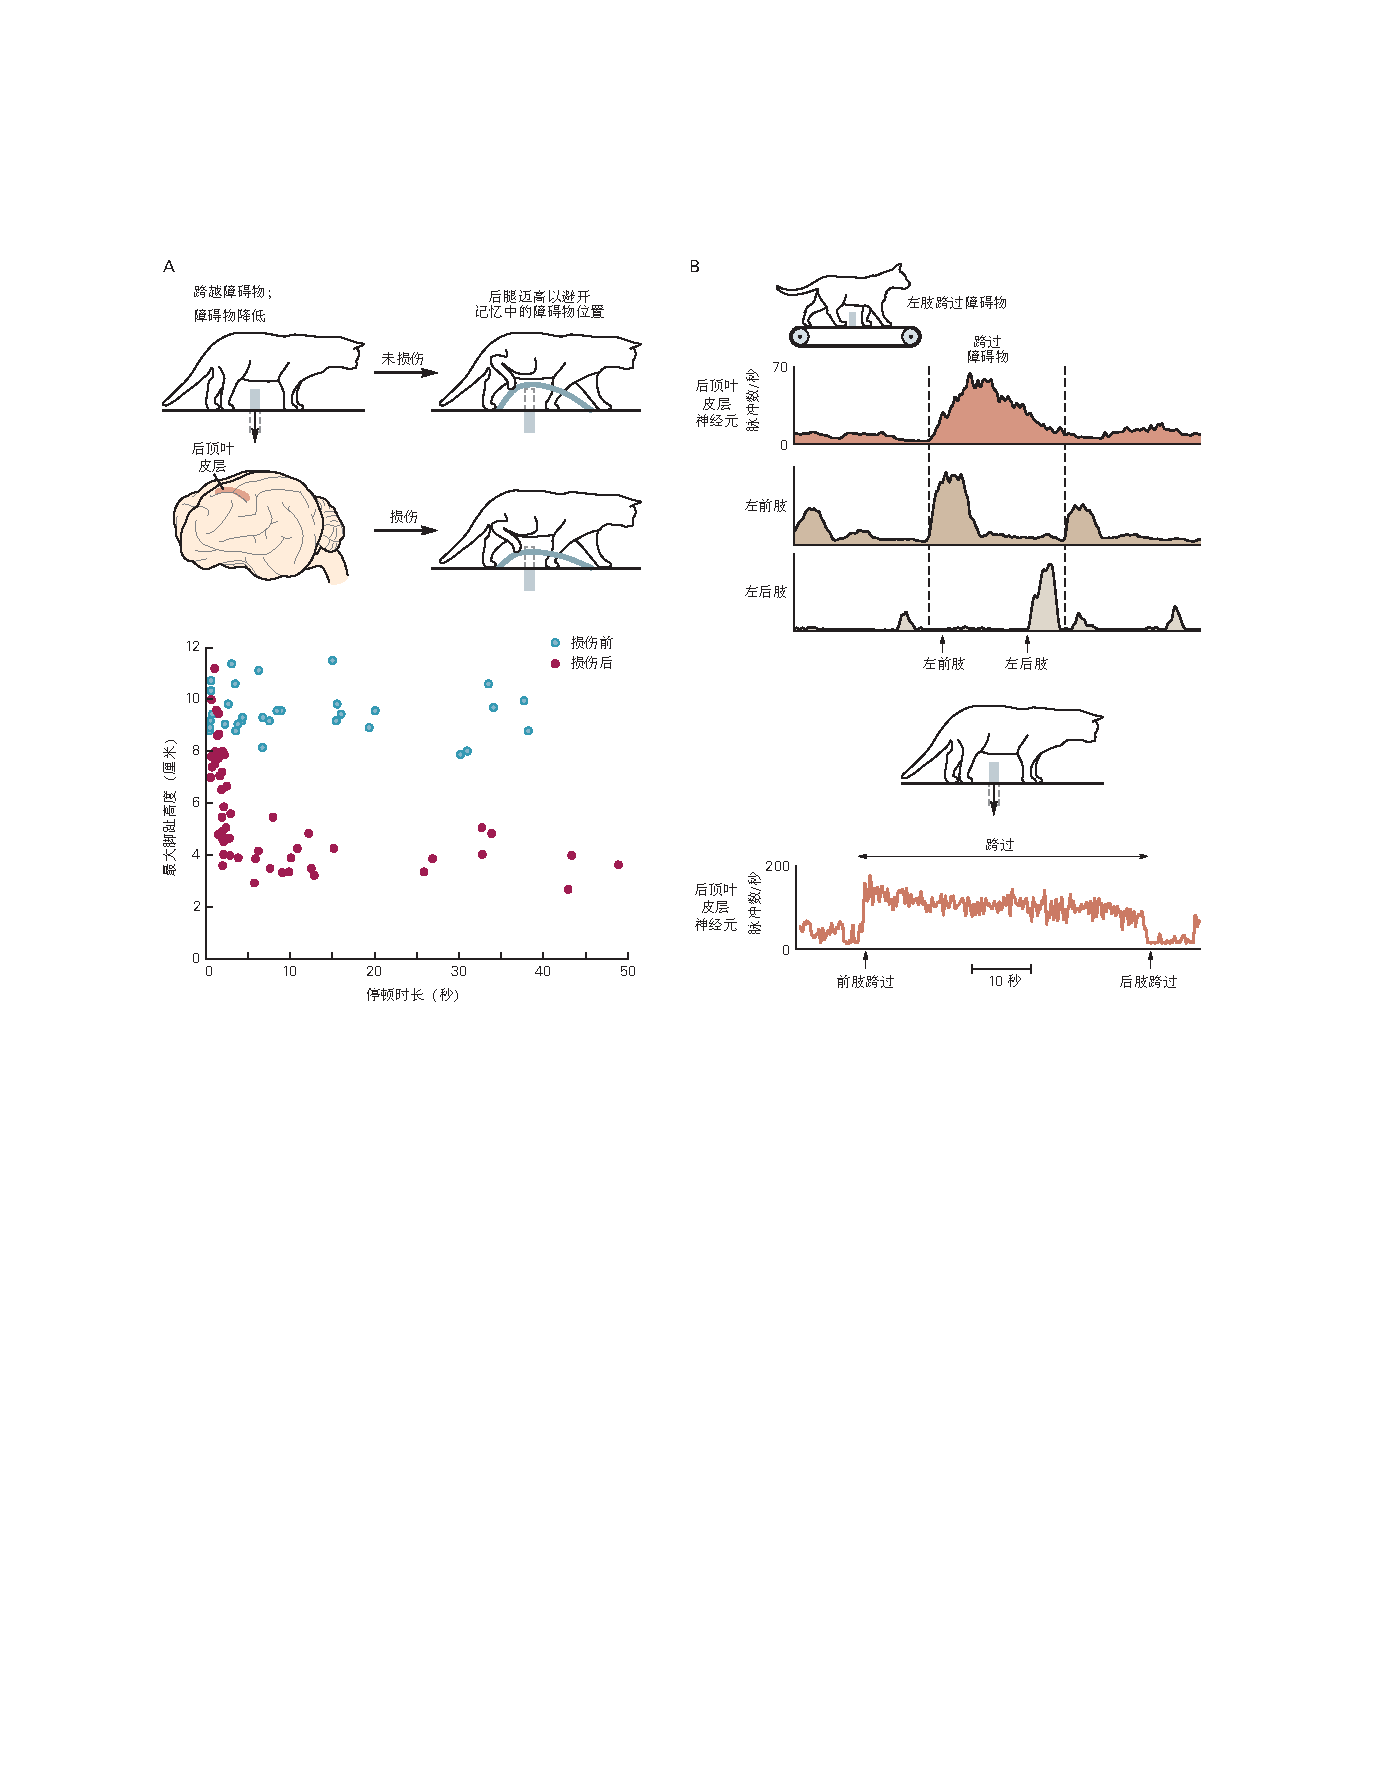
\includegraphics[width=0.95\linewidth]{chap33/fig_33_16}
	\caption{后顶叶皮层 (PPC) 参与维持运动过程中工作记忆障碍的估计。 A. 上图:训练正常动物向前走,跨过障碍物,然后停下来。 当动物停下来时,障碍物被移除了。 当重新开始行走时,后腿抬高以避开记忆中的障碍物。 这段记忆持续了三十多秒。 后肢的轨迹根据障碍物的高度和后爪的相对位置进行了适当的缩放。 PPC 的双侧损伤导致记忆力受损,使得动物不可能在不撞到障碍的情况下通过障碍。 下图:损伤后,动物仅储存了 1 至 2 秒的记忆,脚趾的最大高度不足以清除障碍物,明显低于损伤前状态。 (改编自 McVea 和 Pearson 2009。)B. 上图:记录在完整动物的右侧 PPC 中的神经元在左前肢 (lFL) 和后肢 (lHL) 通过障碍物之间的期间放电 ( 由每个肢体中代表性屈肌的肌电图活动表示)。 这种放电可用于在视觉引导步态修改期间协调后肢与前肢的运动。 下图:当猫跨过障碍物并停下来时,如 A 部分所示,PPC 中的细胞显示出持续的放电,可以提供工作记忆的神经表征。 (经许可改编自 Lajoie 等人,2010 年。)}
	\label{fig:33_16}
\end{figure}



\section{小脑调节下行信号的时间和强度}

小脑损伤导致运动运动明显异常,包括需要加宽支撑基、关节协调受损以及步进时四肢之间的异常耦合。
这些症状是共济失调的特征(第 \ref{chap:chap37} 章),表明小脑对运动的调节起着重要作用。


小脑的一个主要功能是根据发送到脊髓的运动信号与该运动命令产生的运动的比较来纠正运动(第 \ref{chap:chap37} 章)。
在运动的背景下,运动信号由运动皮层和脑干核团中的神经元产生。
有关运动的信息来自上升的脊髓小脑通路。
对于猫的后腿,这些是背侧和腹侧脊髓小脑束。
背侧脊髓小脑束中的神经元(DSCT 神经元)被许多腿本体感受器强烈激活,从而为小脑提供有关后腿机械状态的详细信息。
相比之下,腹侧神经元(VSCT 神经元)主要由 CPG 中的中间神经元激活,从而为小脑提供有关脊髓运动网络状态的信息。


在运动过程中,运动命令(中枢输出副本)、运动(传入副本,通过 DSCT)和脊柱网络的状态(脊髓输出副本,通过 VSCT)在小脑内整合并表示为 小脑皮层中浦肯野细胞和小脑深部核团神经元节律性放电模式的变化。
这些来自小脑深部核团的信号随后被发送到运动皮层和各种脑干核团,在那里它们调节下行信号到脊髓以纠正任何运动错误。


行为实验表明,小脑在步态适应中也起着重要作用。
例如,当受试者在分开的跑步机上行走时,每条腿以不同的速度行走,他们最初表现出非常不对称的步态,然后随着时间的推移适应更不对称的步态。
当两条跑步机带重置为相同速度时,它们再次显示不对称步态,表明实验条件已产生适应性(见图 30-13)。
小脑受损的患者无法适应这种情况。


\section{基底神经节改变皮质和脑干回路}

基底神经节存在于从最古老的脊椎动物到灵长类动物的所有脊椎动物中,可能有助于选择不同的运动模式。
在帕金森病患者身上观察到的运动缺陷清楚地证明了基底神经节对运动控制的重要性,由于来自黑质的多巴胺能输入退化,基底神经节的正常功能受到破坏(第 \ref{chap:chap38} 章)。


此类患者表现出缓慢、缓慢的步态特征,并且在疾病的后期阶段,还可能表现出“僵硬”的步态。
帕金森病患者在运动过程中也表现出平衡问题,以及在步态模式开始时发生的预期姿势调整。
这些缺陷表明基底神经节有助于启动、调节和修改步态模式。
这种调节是由基底神经节向脑干通路和皮质结构的两个主要投射介导的。


基底神经节通过投射到 PPN 影响脑干活动。
PPN 从黑质网状部 (SNr) 和苍白球内部 (GPi) 中的 GABA 能抑制神经元接收抑制性输入;
它还接收来自底丘脑核 (STN) 神经元的谷氨酸能输入。
基底神经节对 PPN 的抑制性输入减少和谷氨酸能输入增加被认为可以促进 PPN 的活动并有利于探索性运动。
STN 和 GPi 是深部脑刺激的主要目标,用于改善帕金森病患者的运动症状,例如僵硬和行动不便。


基底神经节通过丘脑连接到额叶皮层的不同部分(包括辅助运动区)来影响皮层活动。
这些连接允许基底神经节对视觉引导的运动发挥调节作用,可能是通过选择不同行为情况所需的适当运动模式。



\section{计算神经科学提供了对运动回路的见解}

虽然功能研究已经揭示了很多关于运动网络的组织,但它们的整体复杂性使得难以捕捉电路的突触和细胞特性的综合功能。
然而,计算网络建模允许人们模拟电路活动并研究电路元件之间的动态相互作用。
可以在多个层面开发计算模型:研究给定回路中神经活动的离子基础,研究特定回路中不同神经元组之间的连通性,或更好地理解运动网络中不同结构之间的相互作用。
每个级别的计算模型都已开发用于研究无脊椎动物和脊椎动物以及从七鳃鳗到哺乳动物的脊椎动物的节律和模式生成。
与其他领域一样,结合实验操作和计算建模的方法在未来几年可能会增加,并有可能增进我们对复杂系统和结构之间相互联系的理解,而这些结构是产生完整运动功能所需的。


\section{人类运动的神经元控制与四足动物相似}

必然地,我们对运动控制背后的神经机制的大部分理解来自对四足动物的实验。
尽管如此,现有证据表明,所有关于四足动物行走的起源和调节的主要原则也适用于人类的运动。
尽管 CPGs 是否存在于人类中的问题仍然存在争议,但一些观察结果与 CPGs 对人类运动很重要的观点是一致的。


例如,对一些脊髓损伤患者的观察结果与脊髓猫的研究结果相似。
在脊髓几乎完全横断的患者中,一些引人注目的病例表明,当臀部伸展时,腿部会出现无法控制的、自发的、有节奏的运动。
这种行为与慢性脊椎猫的有节奏的步进运动非常相似。
此外,与其他哺乳动物一样,对损伤下方的脊髓进行强直电刺激可以引起类似运动的活动。


在脊髓损伤后训练的患者中也发现了人类和四足行走之间的相似之处。
日常训练与药物治疗相结合可以恢复脊柱猫的行走能力,并改善慢性脊柱损伤患者的行走能力。
患有严重脊髓损伤的人已经暴露于跑步机引起的踩踏和药物治疗,类似于那些已被证明可以激活猫的 CPG 的药物治疗,已经证明产生运动的能力有显着改善(方框 33-4)。
这些结果表明 CPG 存在于人类中,并且与其他脊椎动物中发现的 CPG 具有功能相似性。


人类脊柱 CPGs 存在的有力证据也来自对人类婴儿的研究,如果婴儿直立并在水平表面上移动,他们在出生后立即进行有节奏的踏步运动。
这有力地表明,一些用于运动的基本神经元回路是先天的,并且在下行控制系统发育不完善时出生时就存在。
由于缺乏大脑半球(无脑畸形)的婴儿也可能发生步进,因此这些电路必须位于脑干或脑干下方,可能完全位于脊髓内。


在生命的第一年,随着自动踏步转变为功能性步行,这些基本回路被认为受到了脊柱上的控制。
特别是踏步模式,逐渐从产生很少有效向前运动的更原始的屈伸模式发展到复杂动作的成熟模式。
根据对猫的研究,这种适应似乎合理地反映了起源于运动皮层和脑干核团并受小脑调节的下行系统的成熟。


在皮质水平,涉及运动皮质的中风或皮质脊髓束的损伤导致运动缺陷,如猫。
然而,人类的缺陷比猫甚至非人类灵长类动物要严重得多,这表明人类的运动皮层在运动中比其他哺乳动物更重要。
使用经颅磁刺激 (TMS) 调节运动皮层活动的研究还表明,运动皮层对人体运动的控制起着重要作用。
例如,导致皮质失活的 TMS 参数会降低运动期间的肌肉活动水平。
相反,激活运动皮层的 TMS 参数可改善不完全性脊髓损伤后的运动恢复。


成像研究连同高分辨率脑电图记录显示,在运动过程中,尤其是在想象的越过障碍物运动过程中,包括运动皮层、前运动皮层和 PPC 在内的几个皮层区域的活动发生了变化。
成像研究还表明,在运动过程中,中脑那些对动物运动的启动和速度控制很重要的部分的活动增加。
同样,在帕金森病中,脚桥核中的神经元也会受到影响,导致在疾病晚期出现严重的步态障碍。


\section{要点}


1. 运动是一种高度保守的行为,对物种的生存至关重要。
我们对运动产生和控制所涉及的神经元机制的理解最初来自对系统发育较老的动物(例如七鳃鳗和蝌蚪)的研究。
最近,在神经系统更为复杂的哺乳动物中,涉及运动产生和调节的不同神经通路的组织也得到了非常详细的确定。 


2. 脊髓与下行和节律性外周传入输入隔离开来,可以产生复杂的运动模式,其中包含在完整动物身上观察到的节律和模式的元素。
负责产生此活动的电路称为中央模式发生器 (CPG)。 脊髓回路中的活动可以根据经验进行修改。


3. 控制游泳的 CPG 的基本组成部分是产生兴奋性节律的神经元和负责左右交替的连合抑制神经元。
这种组织原则也存在于 CPG 中,通过添加屈肌-伸肌模式生成电路和额外的连合神经元网络来控制四肢运动。
运动网络中的电路具有模块化组织,具有用于组成神经元的不同发射器和分子代码。
下行命令信号作用于这些电路元件以产生运动行为的不同方面。


4. 中间神经元和运动神经元的离子膜特性有助于节律和模式的产生。
对这些特性进行细胞特异性操作将使我们能够准确了解它们对运动生产的相对贡献。


5. 外周传入输入调节脊髓运动回路的功能。
本体感受器用于稳定站立和摆动之间的相变(反之亦然),而来自外部感受器的输入用于修改肢体活动以响应意外扰动。 


6. 参与启动运动、控制运动速度和选择步态的回路位于中脑,包括脚桥核和楔状核中的兴奋性神经元。
这些兴奋性核在控制缓慢的探索性运动或全方位的速度和步态(包括快速逃逸运动)方面发挥着不同的作用。
分子遗传驱动的细胞特异性方法允许无与伦比地访问脑干中这些通路的组织以及它们如何与脊髓运动网络整合。 


7. 脑干中三个主要结构的活动以及下行到脊髓的轴突(桥脑网状结构、外侧前庭核和红核)有助于控制姿势和肢间协调。 来自这些结构的信号以特定于结构的方式改变肌肉活动水平。


8. 运动皮层提供对肌肉活动模式的精确控制,使动物能够在视觉引导下对其步态进行预期调整。
来自运动皮层的信号被整合到正在进行的节奏中。


9. 后顶叶皮层 (PPC) 是网络的一部分,有助于根据视觉信息对步态进行高级规划。
PPC 神经元估计物体相对于身体的相对位置,并在工作记忆中保留信息以促进四肢的协调。 其他皮质和皮质下区域对运动规划的贡献仍然很少研究。


10. 来自小脑和基底神经节的输入用于纠正运动错误并选择适当的运动活动模式。
基底神经节对运动控制的贡献是复杂的,直到现在才被确定。


11. 现有证据表明,通过动物实验确定的神经控制机制也可用于控制人类的运动,包括 CPG 的存在。
在理解脊柱和脊柱上对人类运动控制的影响机制方面仍有待取得重大进展。


12. 最近的技术进步现在给了我们一个无与伦比的机会来研究运动背后的控制机制。
分子和遗传学的进步提供了在细胞和系统水平上操纵行为的能力,并允许详细研究脑干和脊髓回路对运动的启动和调节的贡献。
动物多神经元记录技术的进步,以及人类大脑活动高分辨率记录的发展,将有助于我们理解皮质结构对运动控制的贡献。

